\documentclass[]{formalLabReport}

\usepackage{graphicx}

\usepackage{tikz}

%%%%%%%%%%%%%%%%%%%%%%%%%%%%%%%%%%%%%%%%%%%%%%%%%%%%%%%%%%%%%%%%%%%%%%
% LaTeX Overlay Generator - Annotated Figures v0.0.1
% Created with http://ff.cx/latex-overlay-generator/
% If this generator saves you time, consider donating 5,- EUR! :-)
%%%%%%%%%%%%%%%%%%%%%%%%%%%%%%%%%%%%%%%%%%%%%%%%%%%%%%%%%%%%%%%%%%%%%%
%\annotatedFigureBoxCustom{bottom-left}{top-right}{label}{label-position}{box-color}{label-color}{border-color}{text-color}
\newcommand*\annotatedFigureBoxCustom[8]{\draw[#5,thick,rounded corners] (#1) rectangle (#2);\node at (#4) [fill=#6,thick,shape=circle,draw=#7,inner sep=2pt,font=\sffamily,text=#8] {\textbf{#3}};}
%\annotatedFigureBox{bottom-left}{top-right}{label}{label-position}
\newcommand*\annotatedFigureBox[4]{\annotatedFigureBoxCustom{#1}{#2}{#3}{#4}{white}{white}{black}{black}}
\newcommand*\annotatedFigureText[4]{\node[draw=none, anchor=south west, text=#2, inner sep=0, text width=#3\linewidth,font=\sffamily] at (#1){#4};}
\newenvironment {annotatedFigure}[1]{\centering\begin{tikzpicture}
\node[anchor=south west,inner sep=0] (image) at (0,0) { #1};\begin{scope}[x={(image.south east)},y={(image.north west)}]}{\end{scope}\end{tikzpicture}}
%%%%%%%%%%%%%%%%%%%%%%%%%%%%%%%%%%%%%%%%%%%%%%%%%%%%%%%%%%%%%%%%%%%%%%


\graphicspath{ {./report-images/} }
\begin{document}

\title{Electronics Online Challenge}
\author{Raider Robotics - MSOE1}
\submissionDate{12/7/2020}

\maketitle

\tableofcontents

\newpage

\section{Introduction}
For this challenge, we chose to disassemble a Segway i2 SE PT. One of our teammates obtained 
the Segway in non-working condition and is currently trying to rebuild the electronics to add
features to the device. We decided that this challenge would provide an excellent opportunity for
us to gain a much better understanding to the proprietary systems inside of the device, and understand
the engineering that makes the devices as robust as they are.

\section{Summary and Findings}
The Segway contains two main processing boards, which are identical mirrors. The processing board was
originally covered in a waterproof conformal coating to protect the electronics, which we removed selectively.
We found an array of chips and other components, and will attempt to classify them according to 
three different states of background information:
\begin{enumerate}
    \item \textbf{Fully Classified:} Data for the exact component was obtained
    \item \textbf{Partly Classified:} Data for another components of the same package type and similar ID were obtained
    \item \textbf{Not Classified:} No data for the given component could be obtained
\end{enumerate}

\section{Conclusion} 

\begin{figure}
    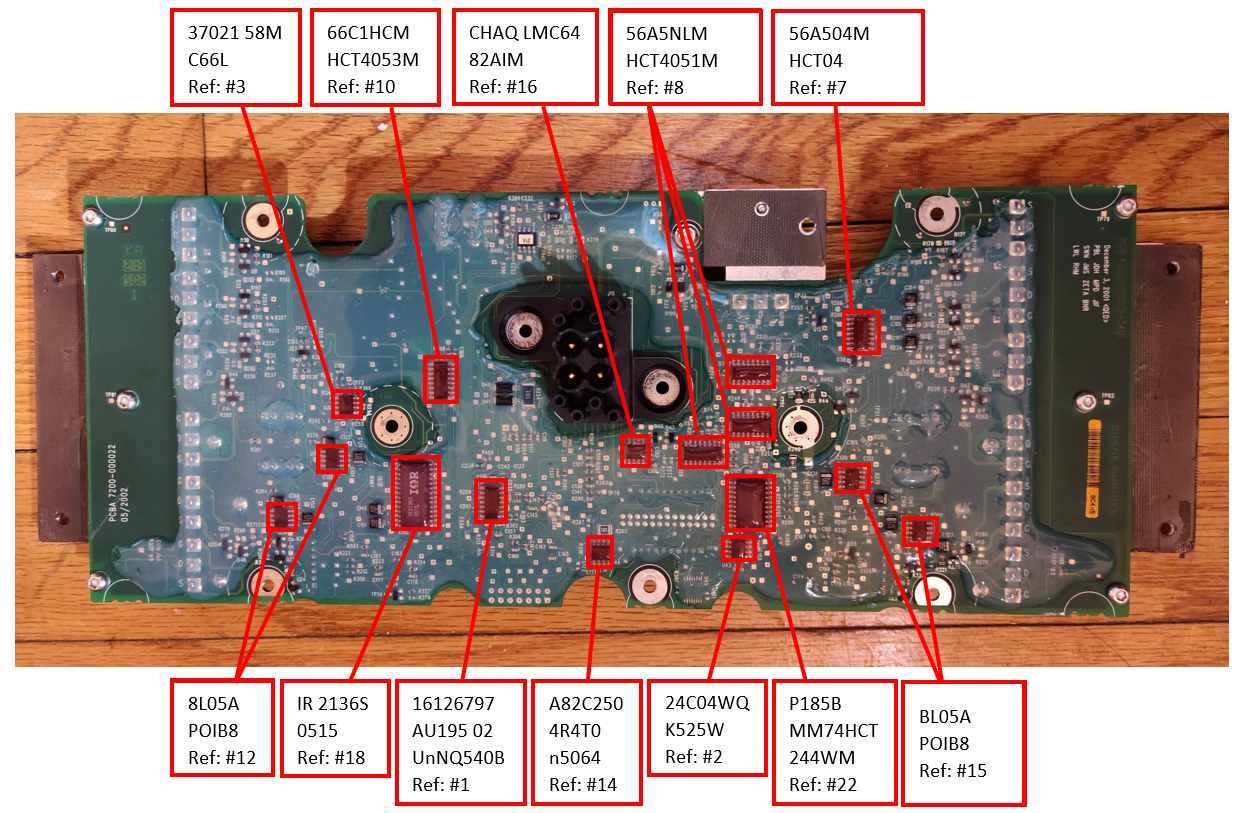
\includegraphics[]{annotatedBoardBack.png}
    \caption{caption}
    \label{fig:annotatedBoardBack.png}
\end{figure}

\begin{figure}
    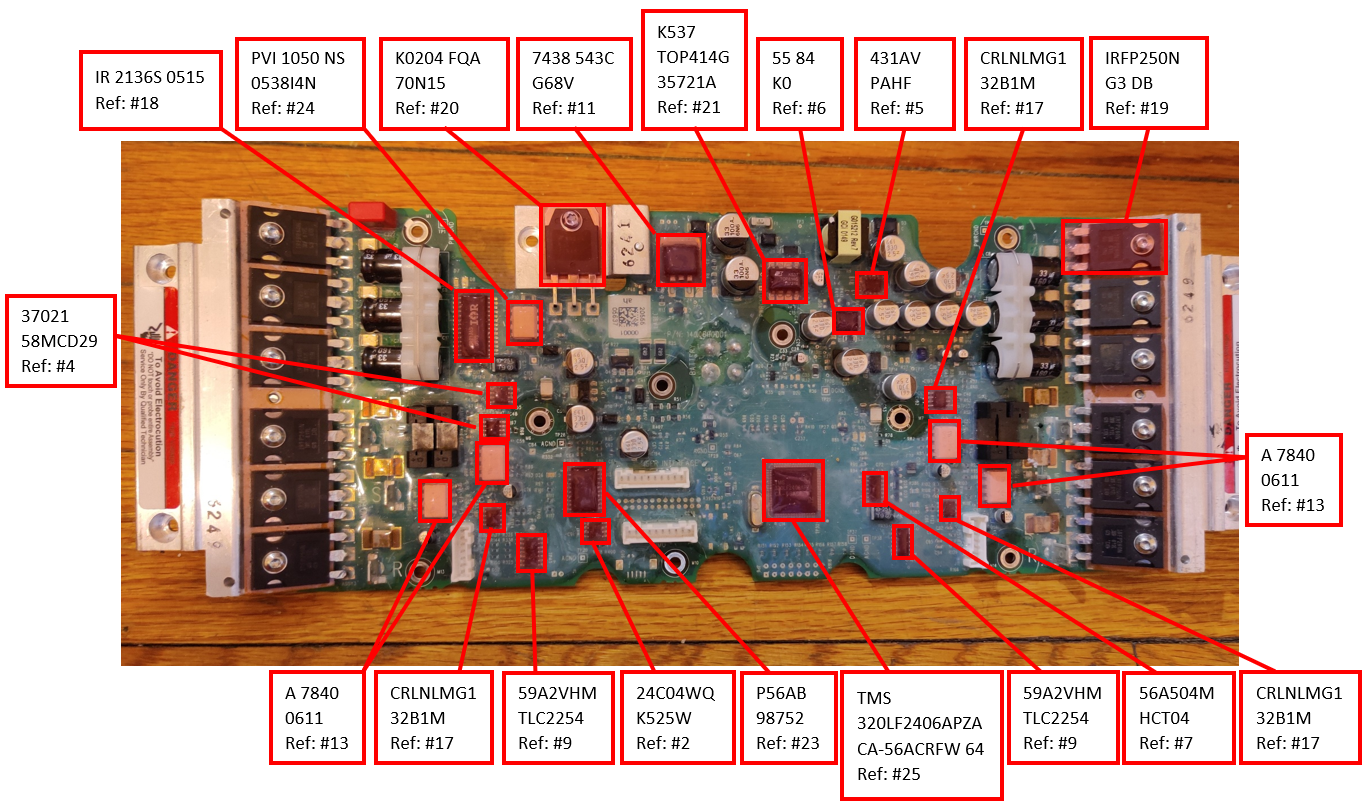
\includegraphics[]{annotatedBoardFront.png}
    \caption{caption}
    \label{fig:annotatedBoardFront.png}
\end{figure}

\begin{figure}
    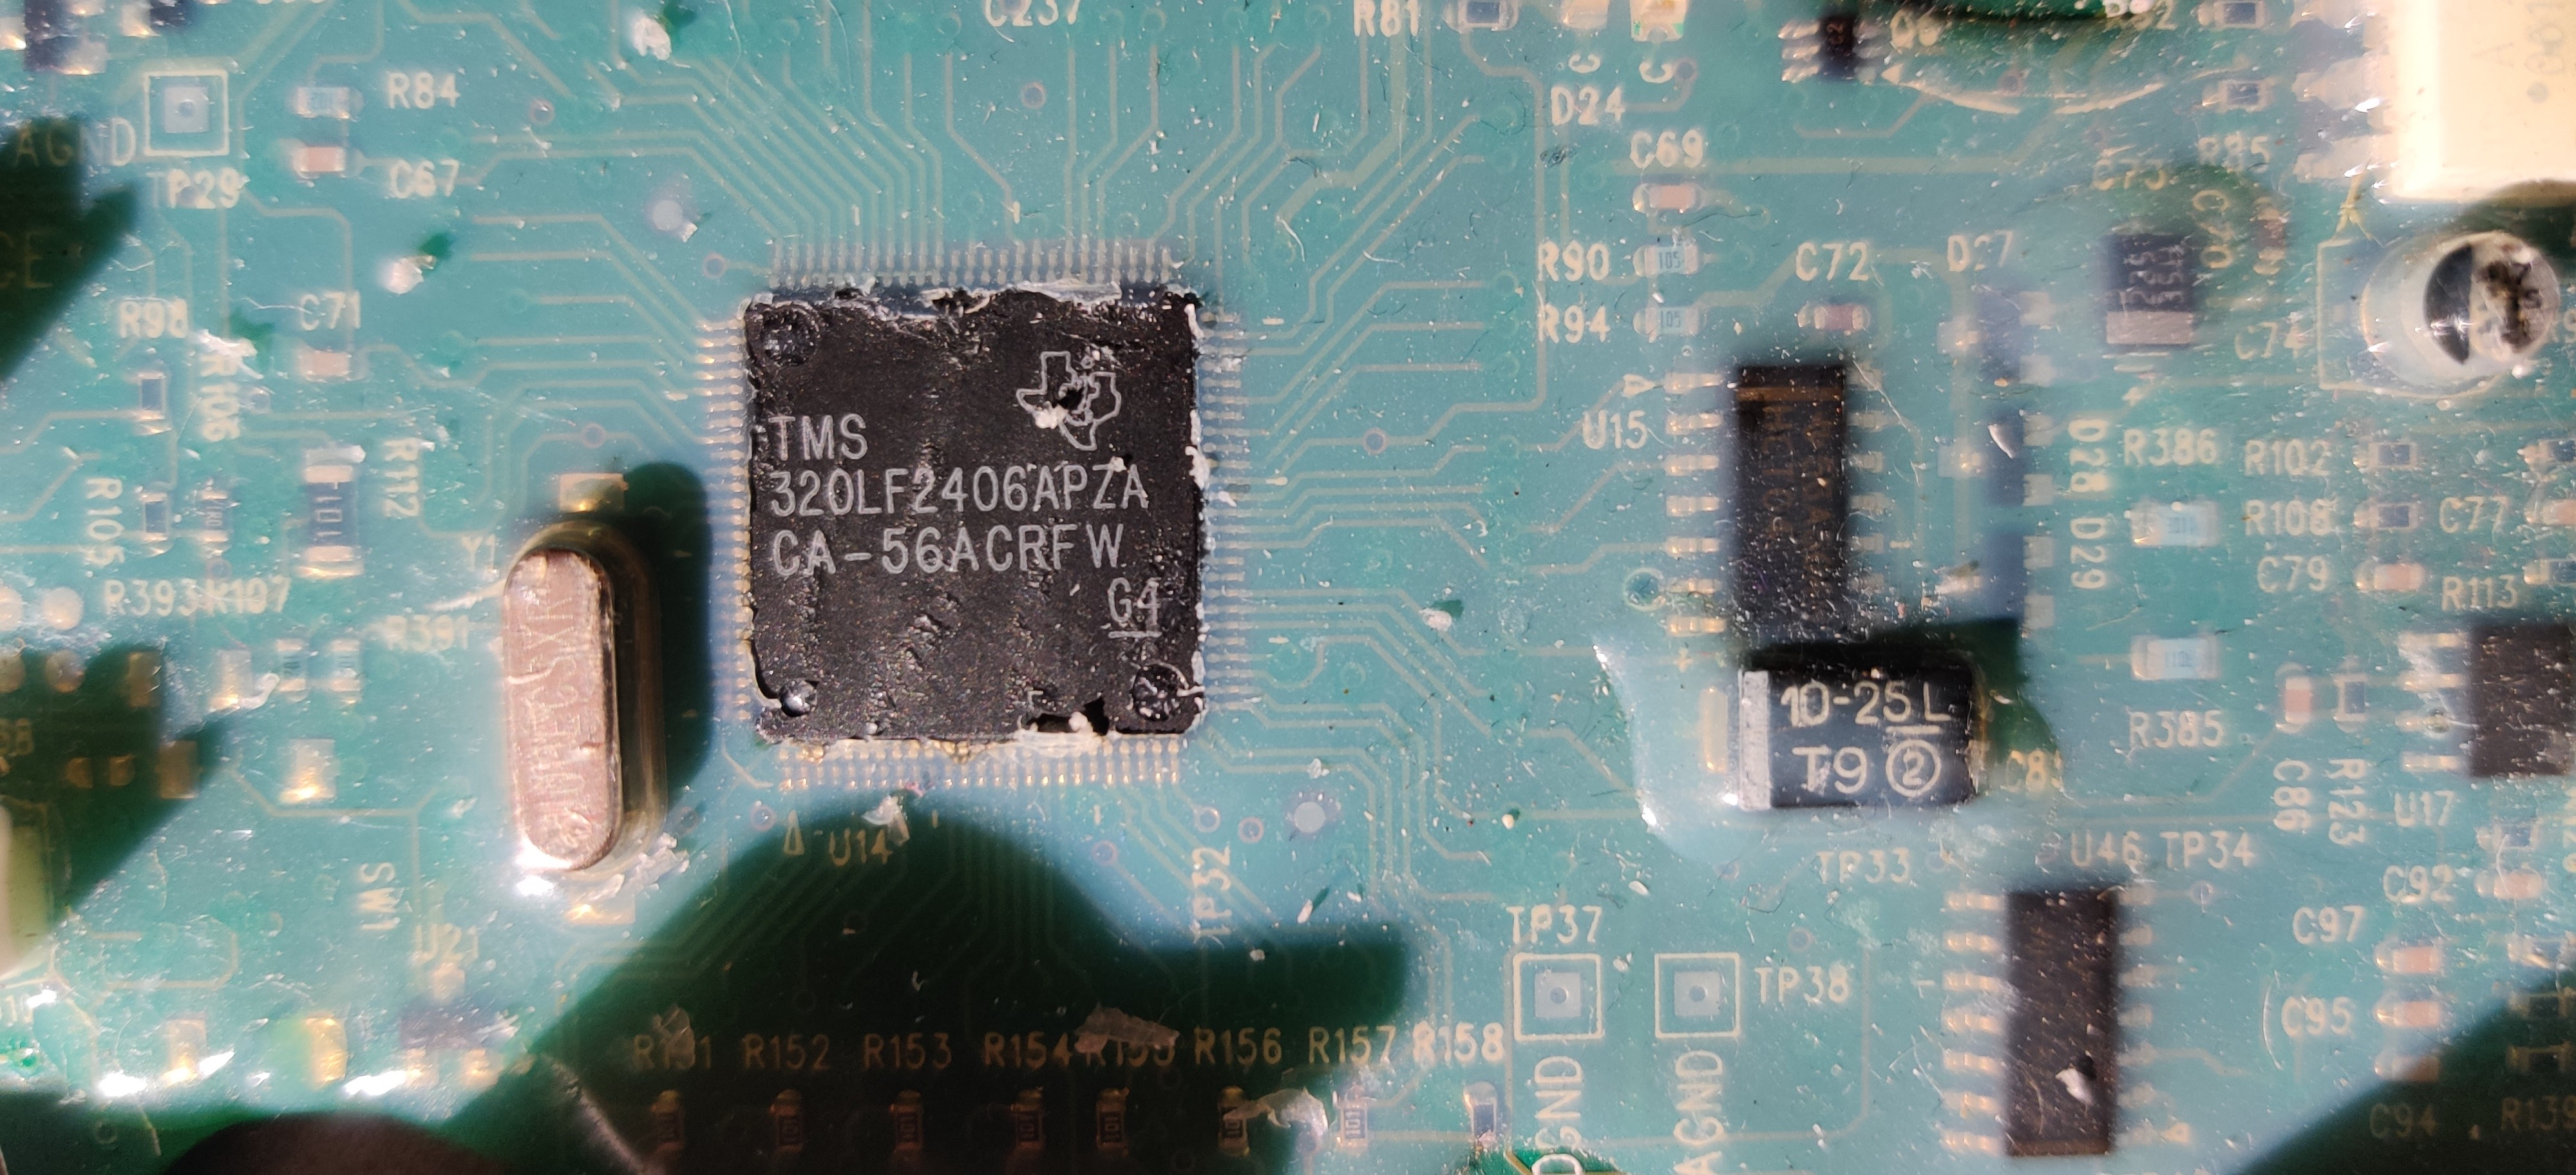
\includegraphics[]{chipImg-320LF2406APZA.jpg}
    \caption{caption}
    \label{fig:chipImg-320LF2406APZA.jpg}
\end{figure}

\begin{figure}
    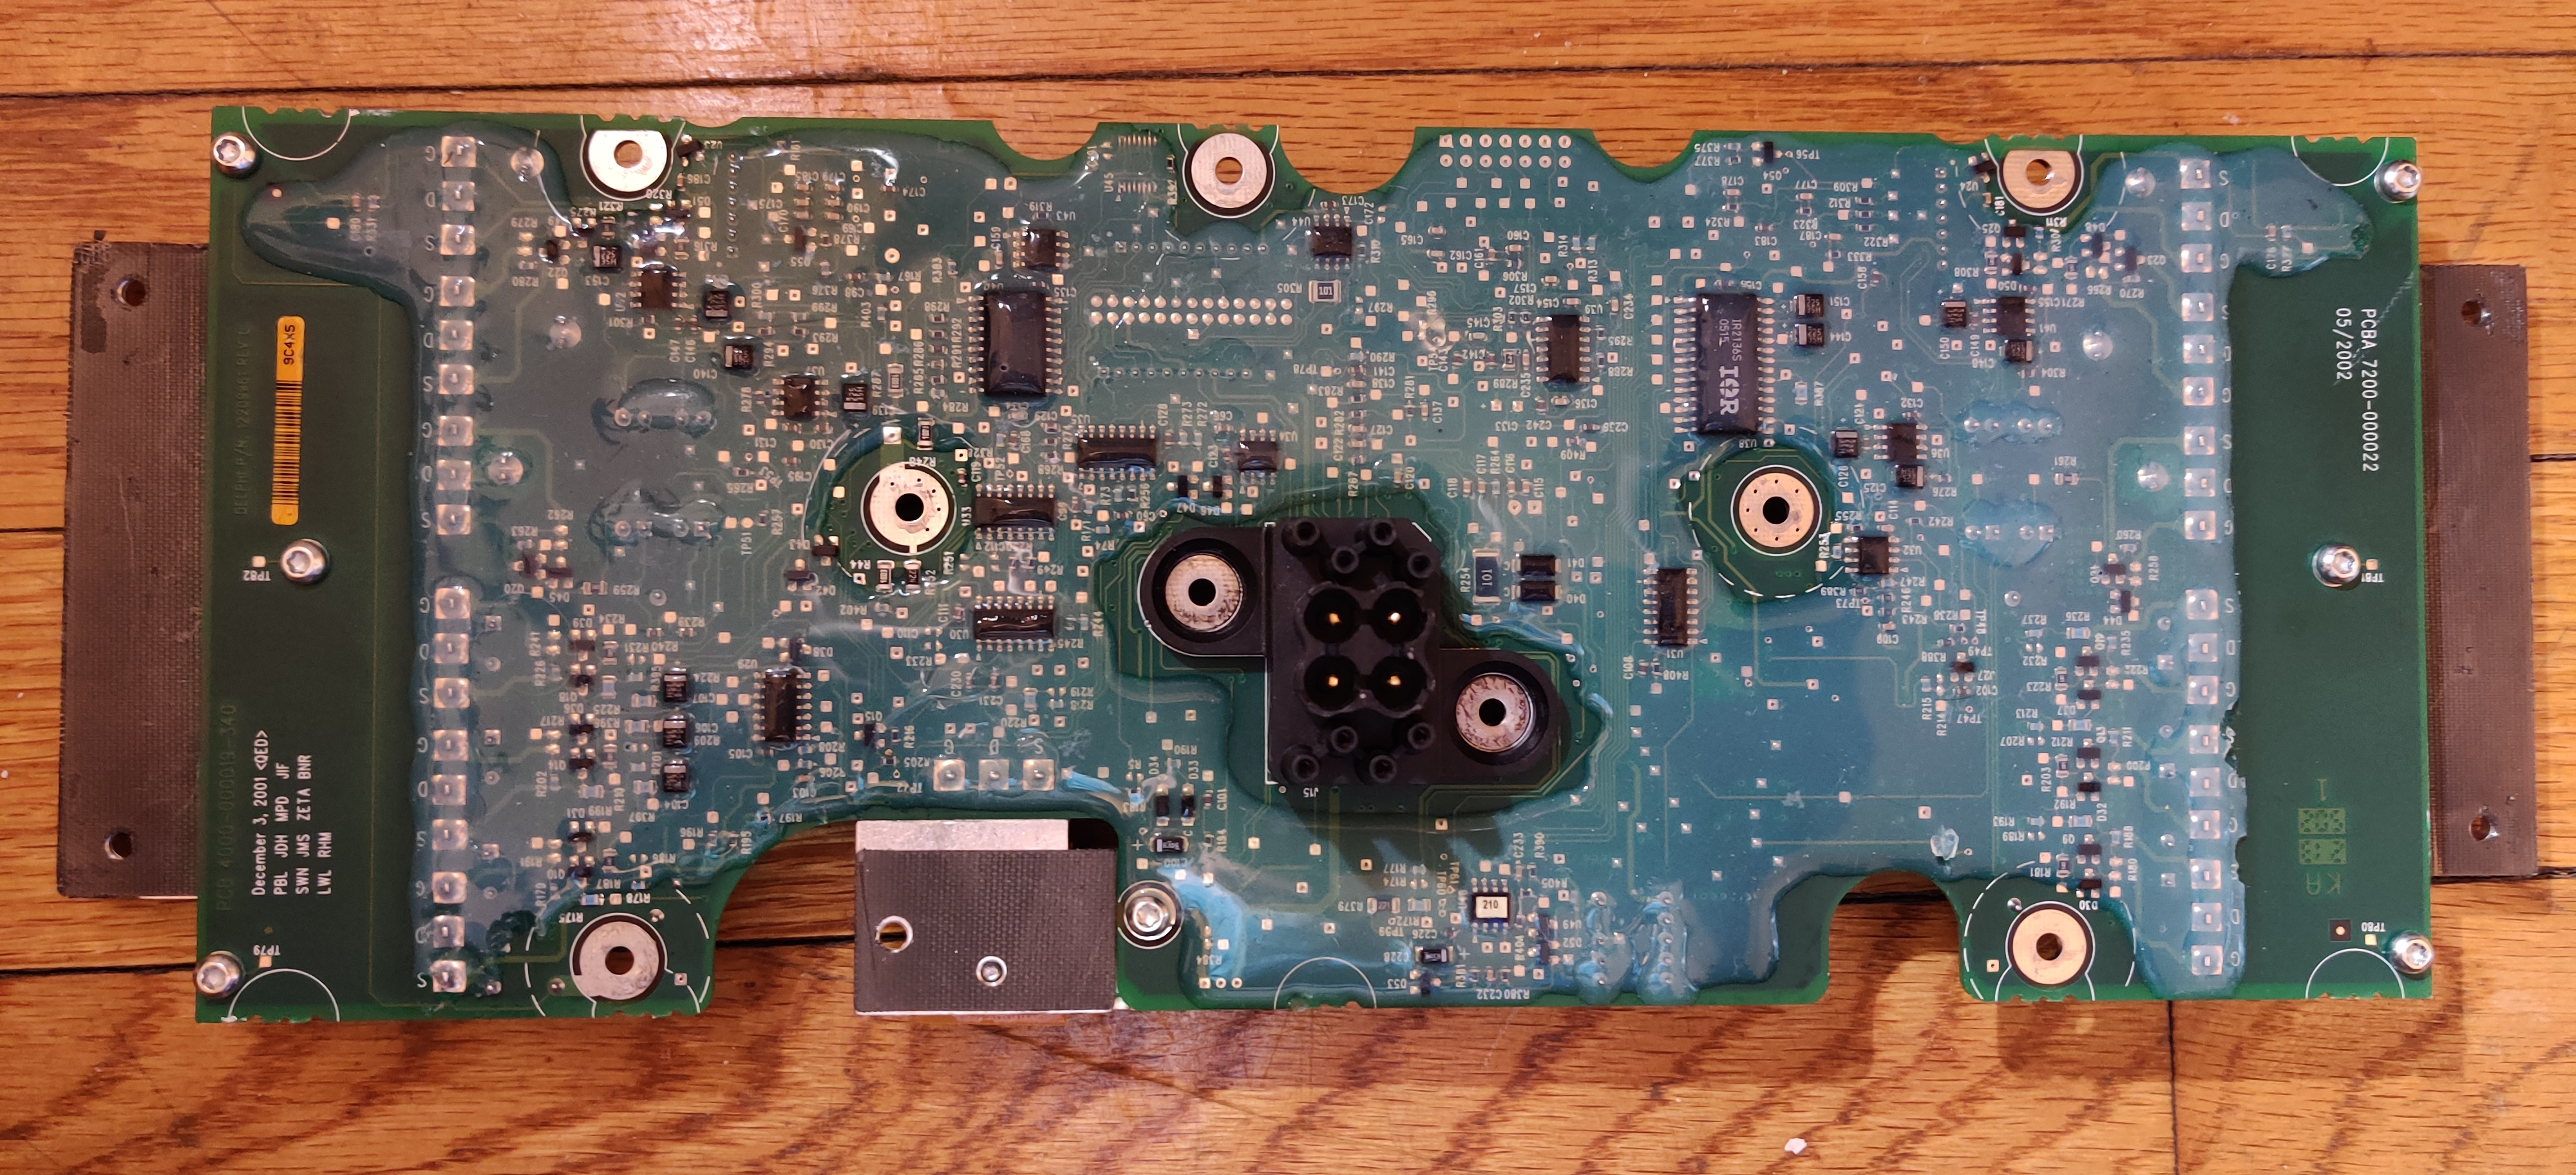
\includegraphics[]{entireBoardBottom.jpg}
    \caption{caption}
    \label{fig:entireBoardBottom.jpg}
\end{figure}

\begin{figure}
    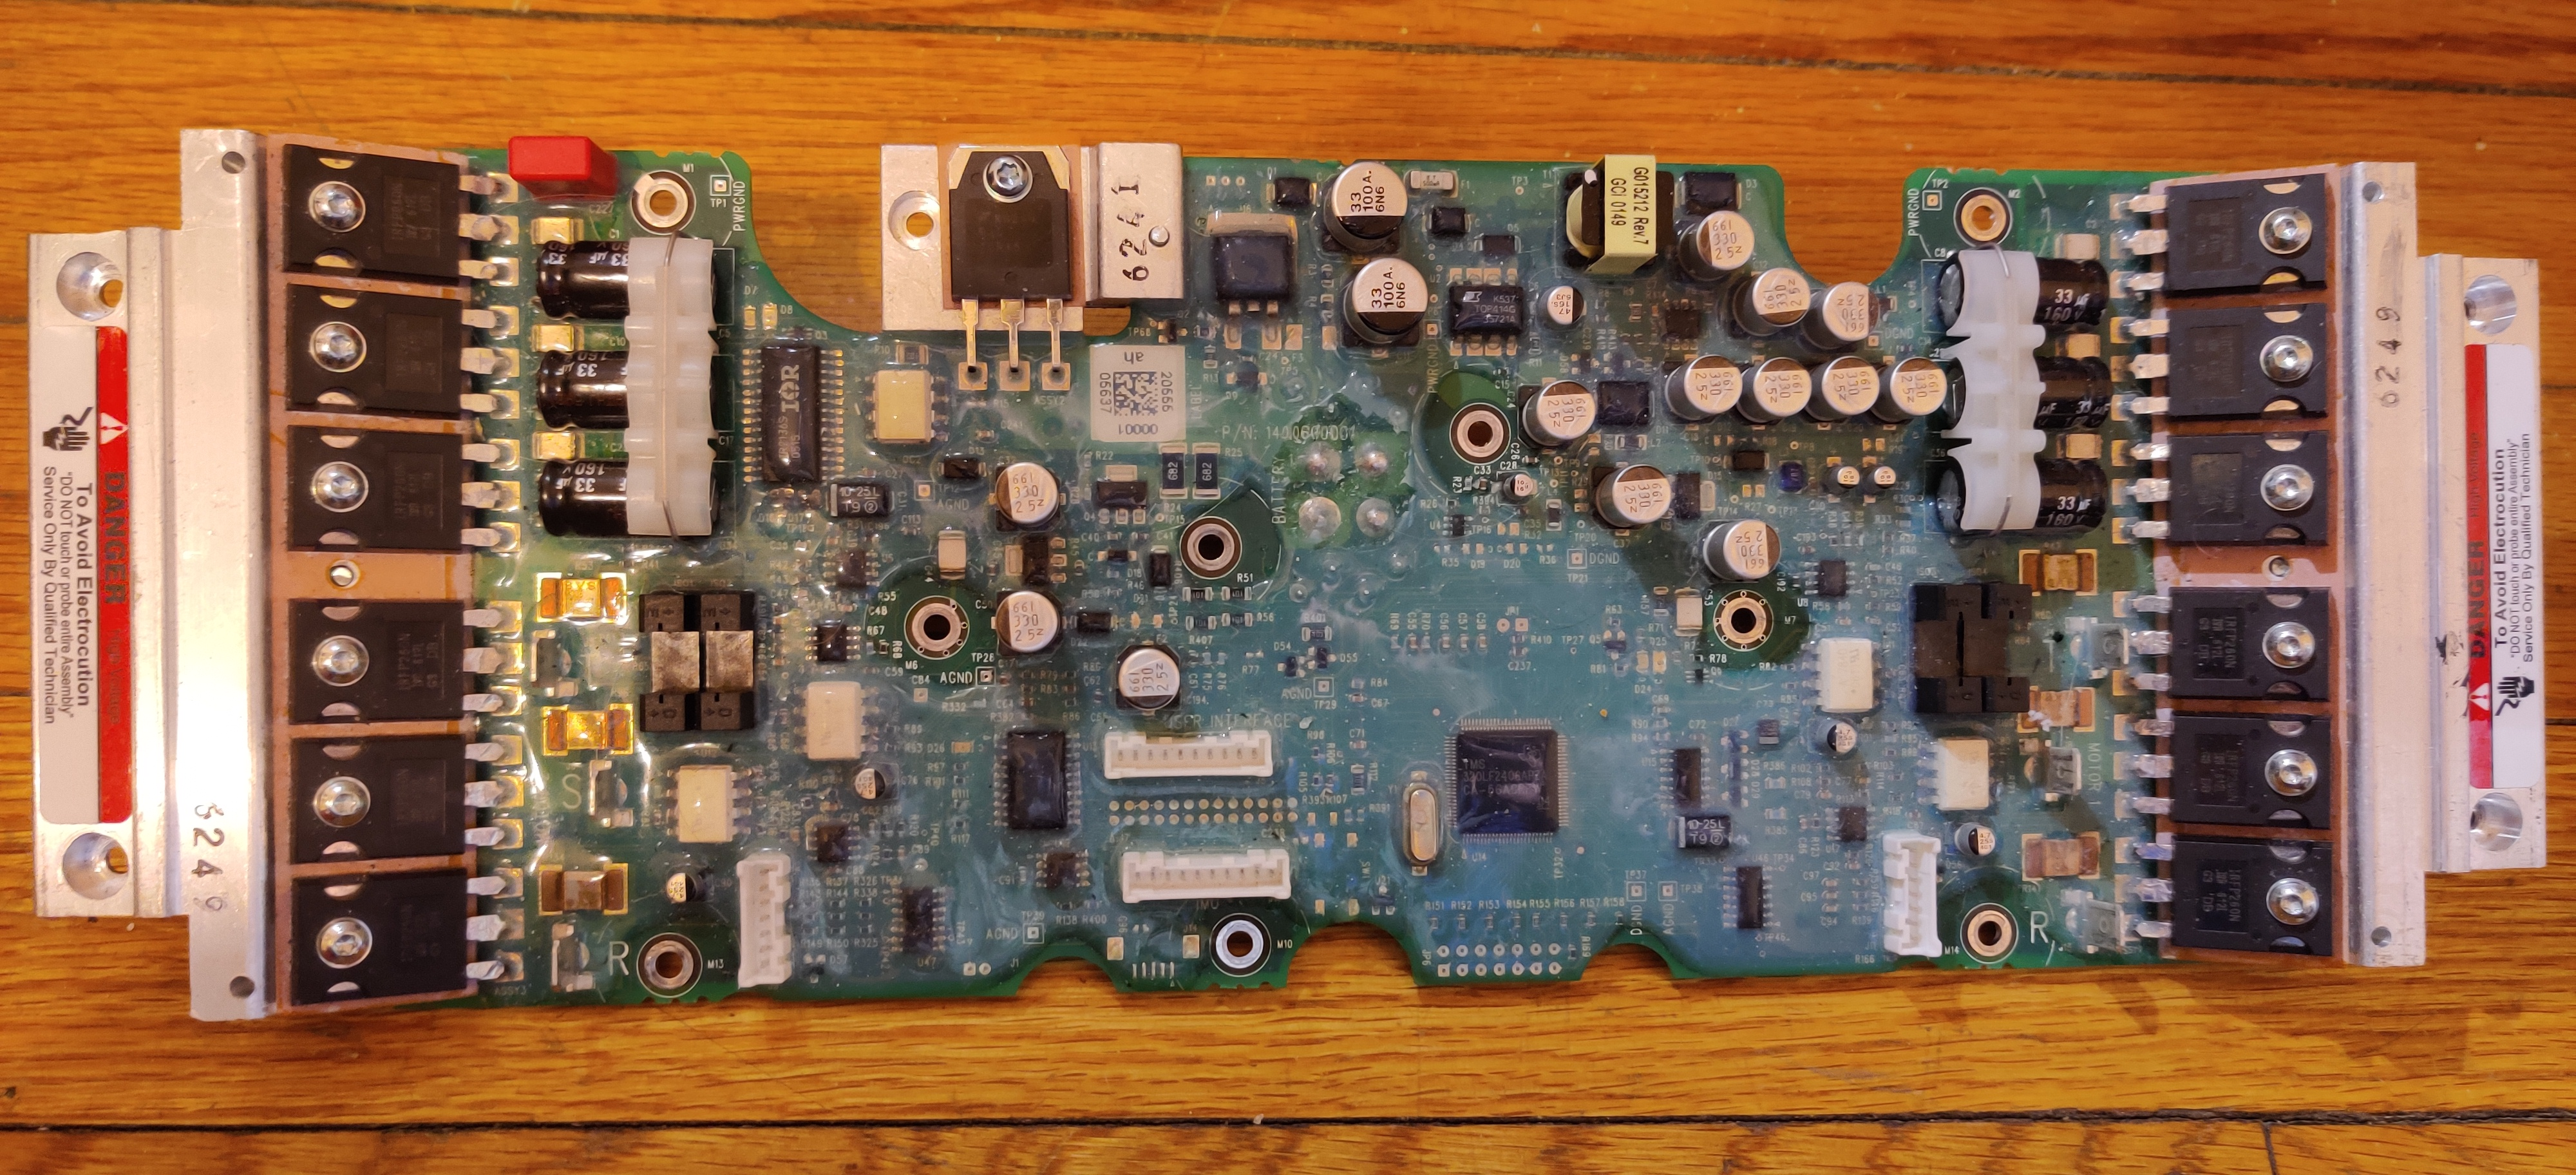
\includegraphics[]{entireBoardTop.jpg}
    \caption{caption}
    \label{fig:entireBoardTop.jpg}
\end{figure}

\begin{figure}
    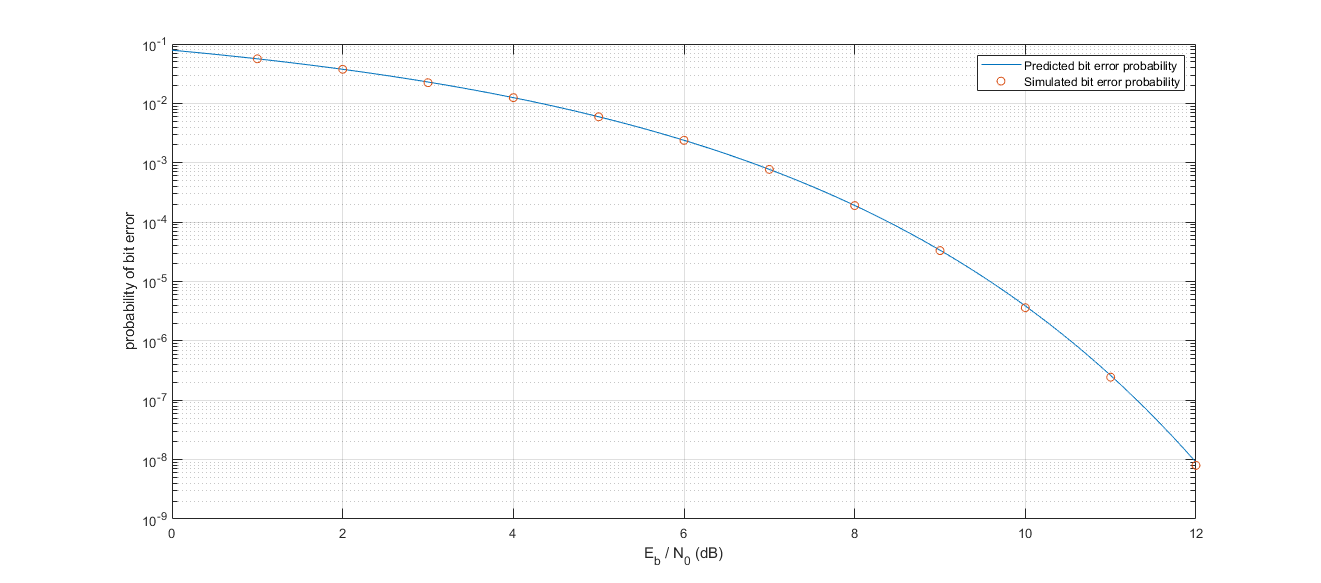
\includegraphics[]{report.png}
    \caption{caption}
    \label{fig:report.png}
\end{figure}

\begin{figure}
    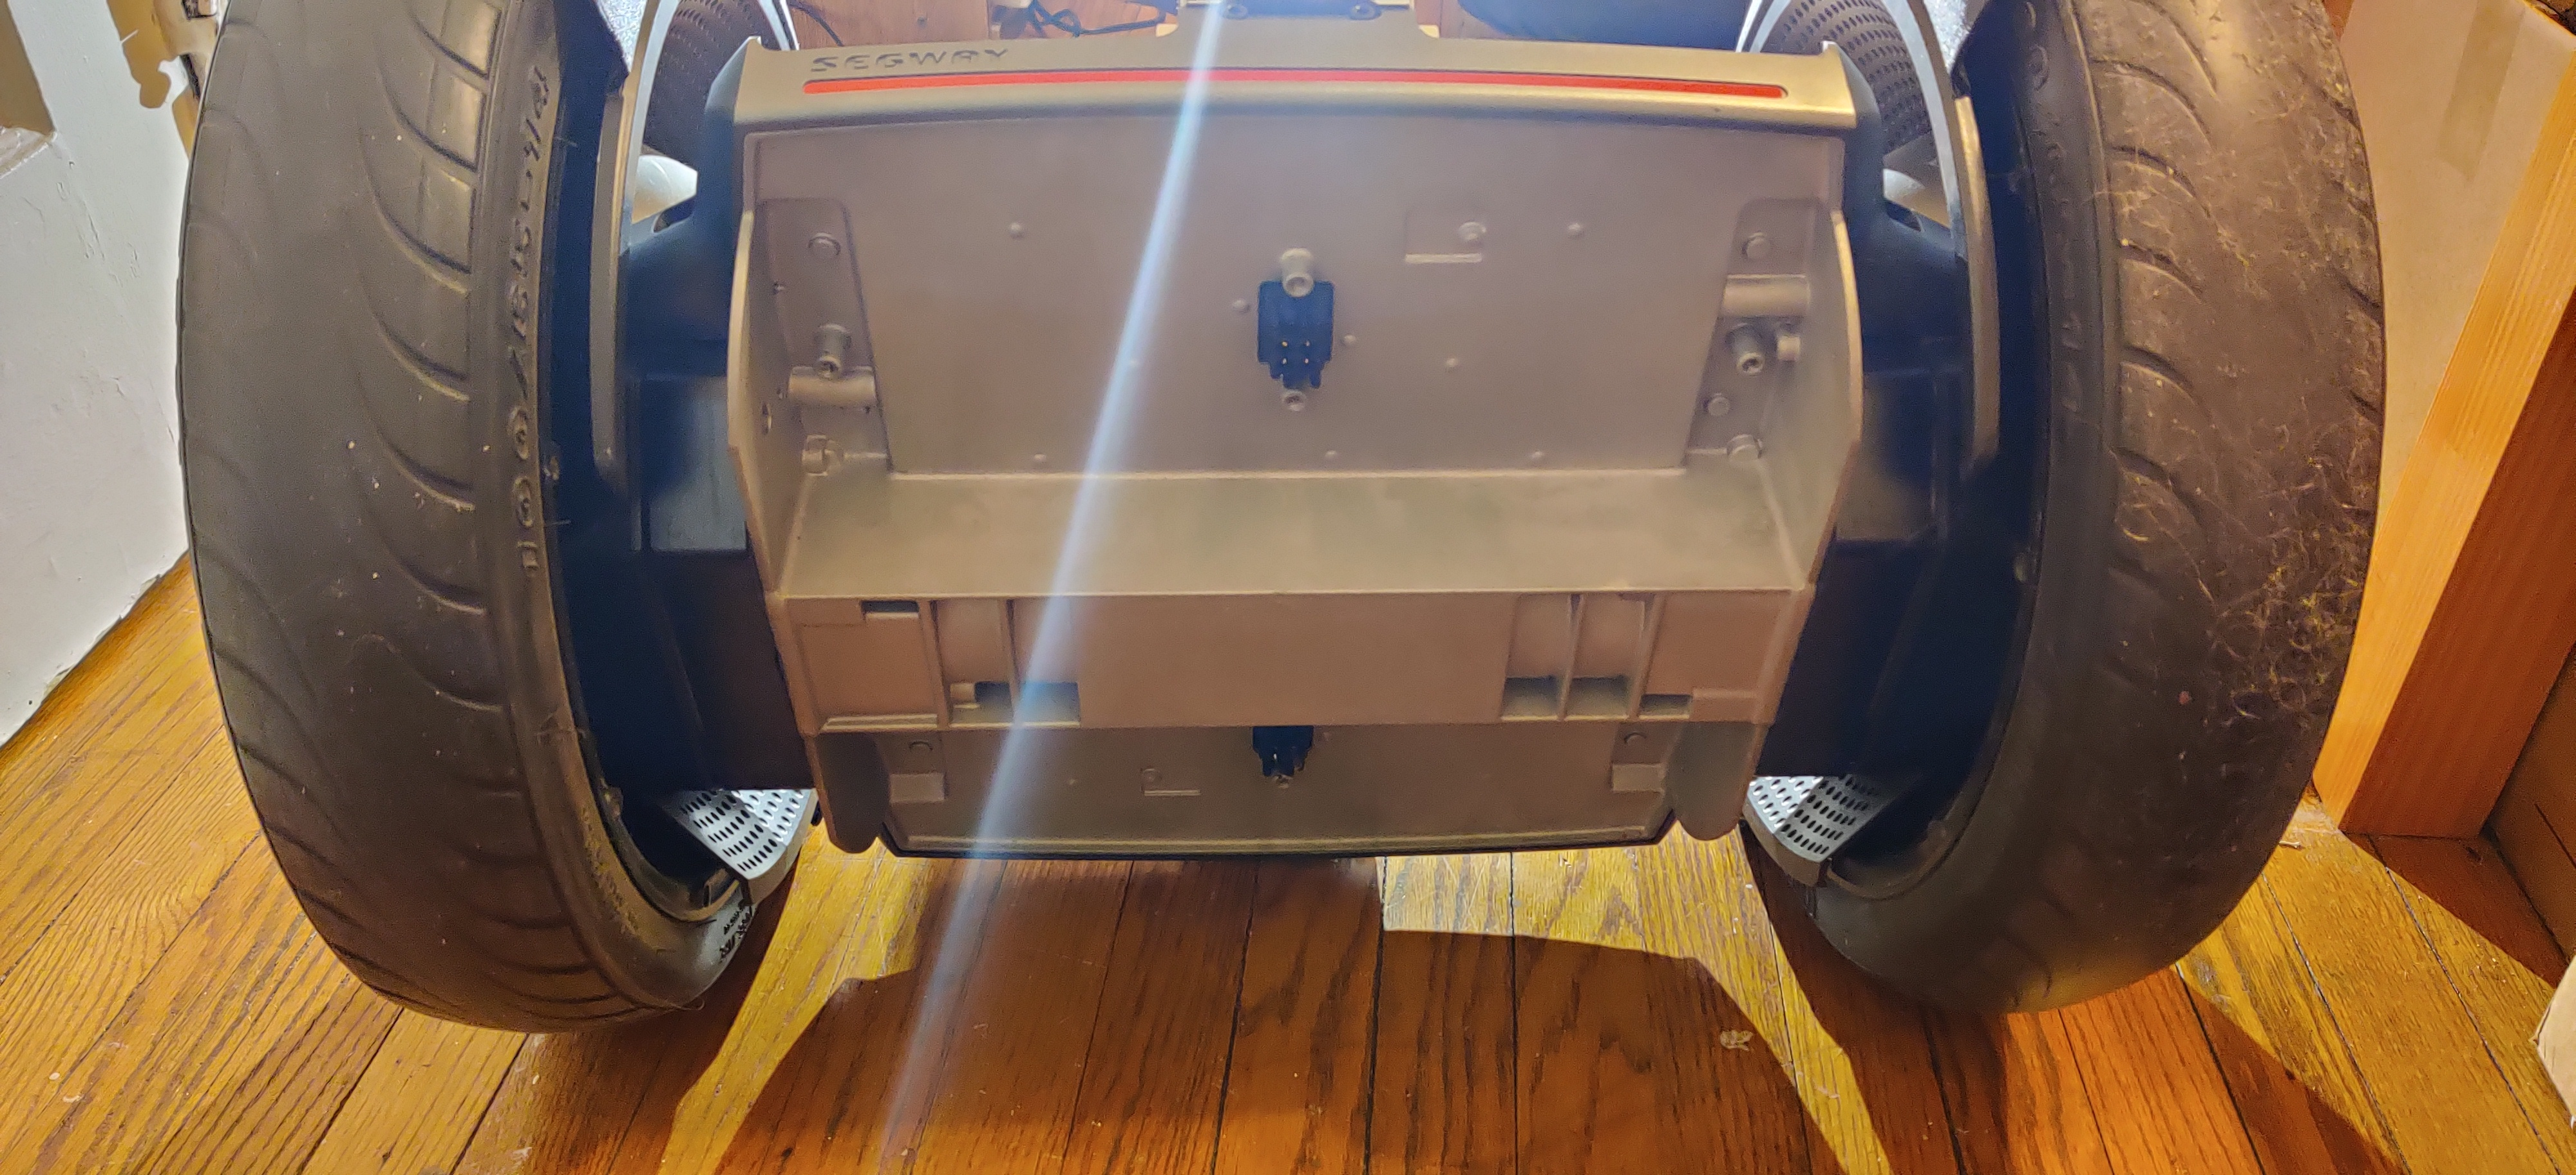
\includegraphics[]{segwayBottom.jpg}
    \caption{caption}
    \label{fig:segwayBottom.jpg}
\end{figure}

\begin{figure}
    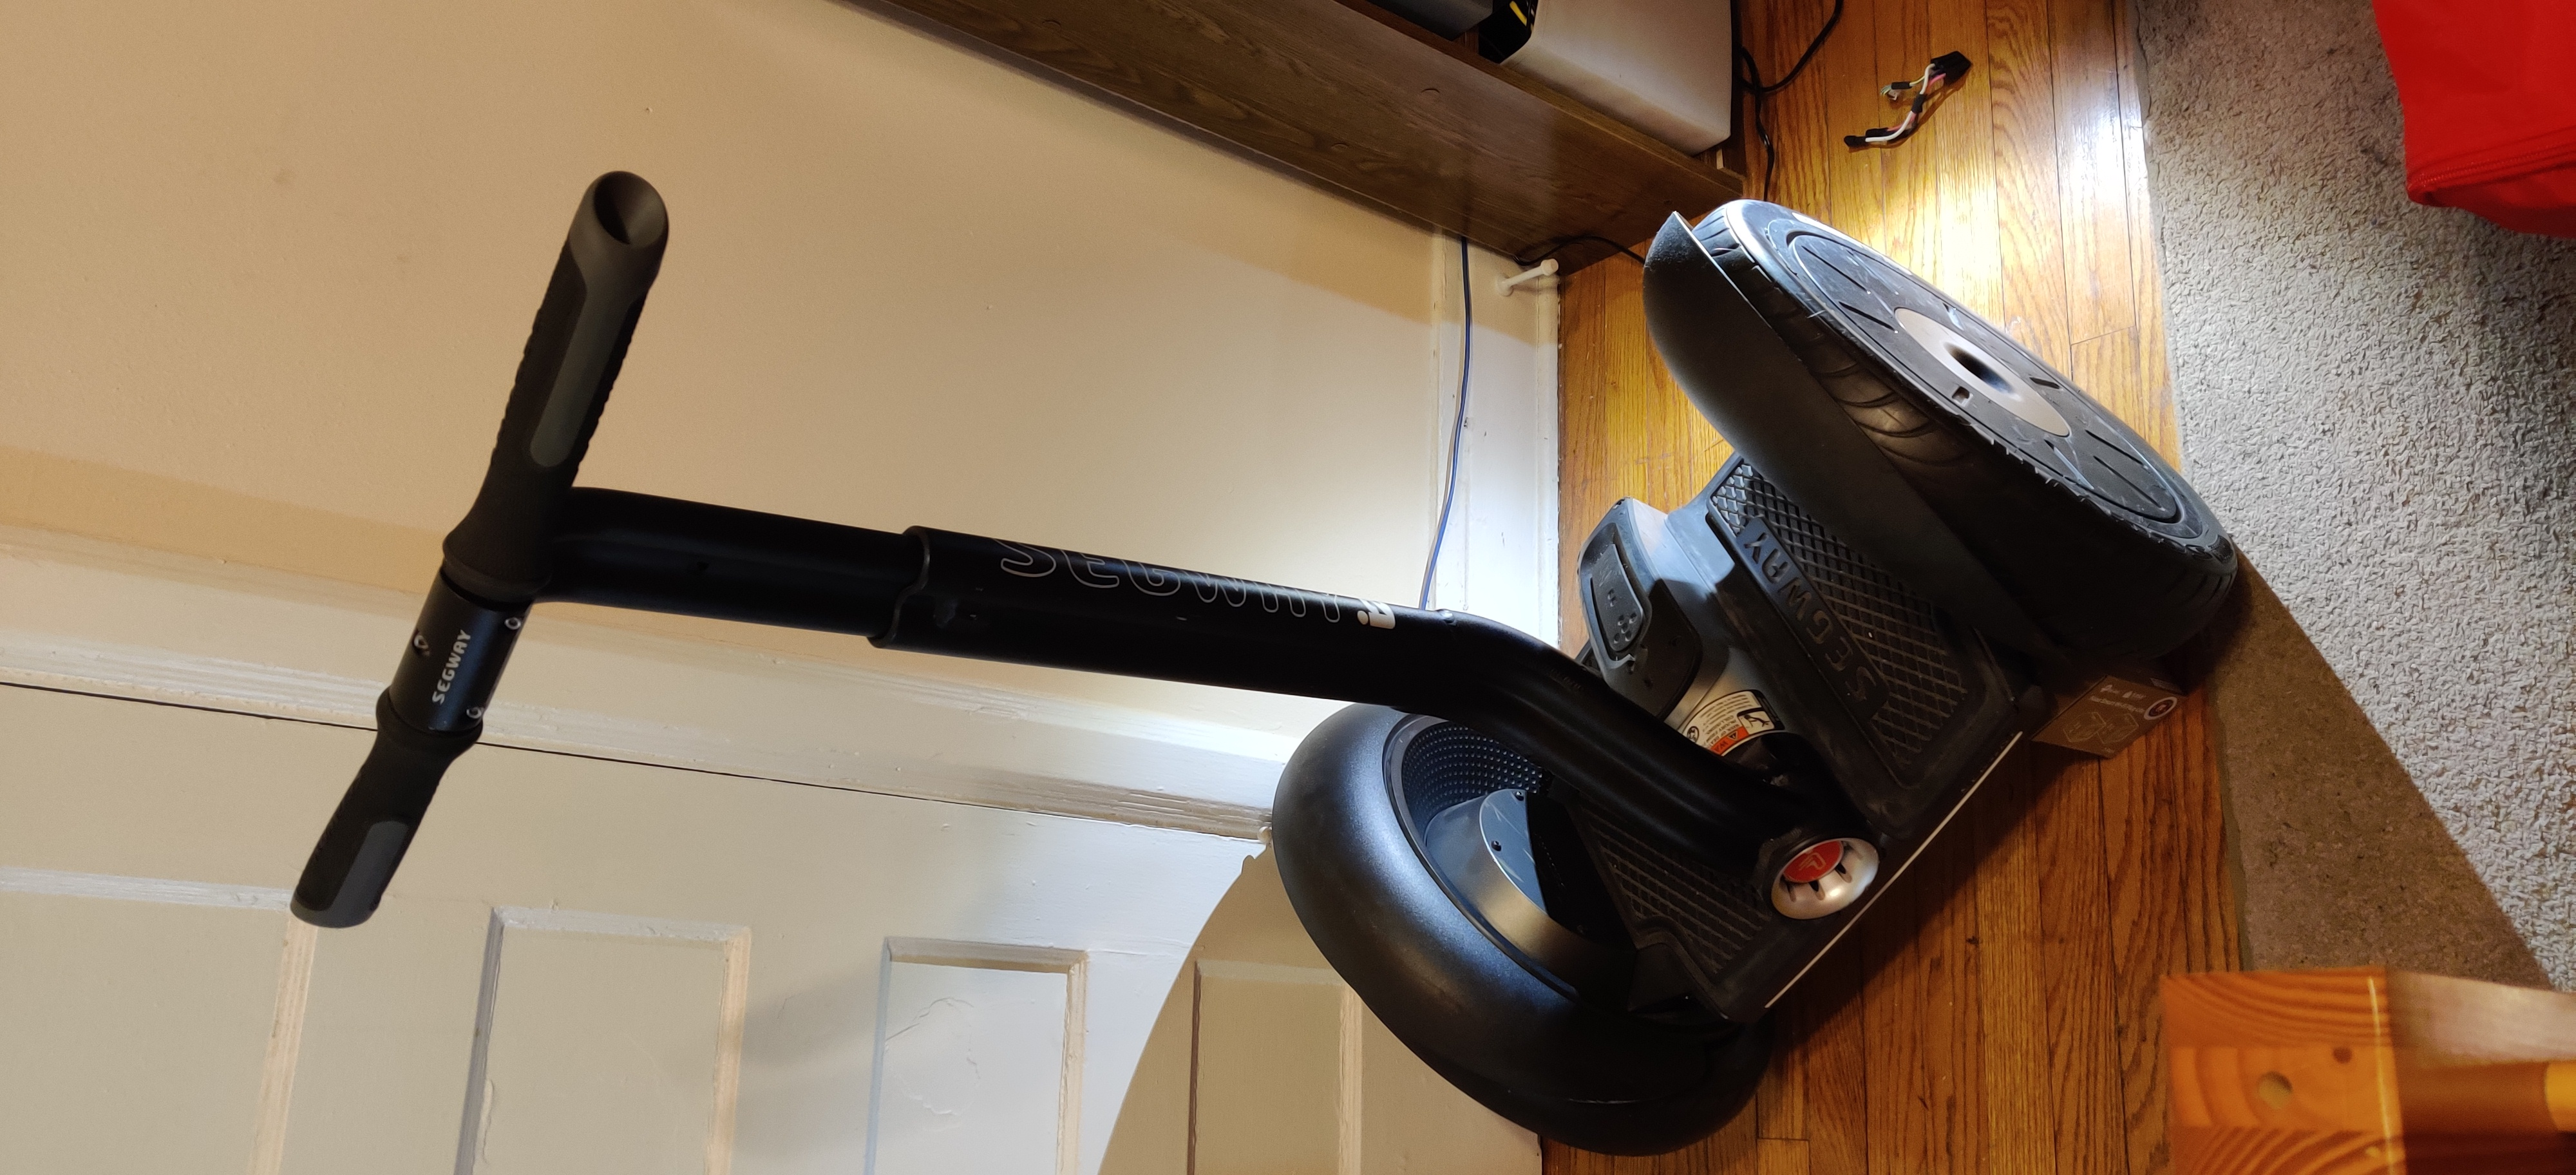
\includegraphics[]{segwayFront.jpg}
    \caption{caption}
    \label{fig:segwayFront.jpg}
\end{figure}

\begin{figure}
    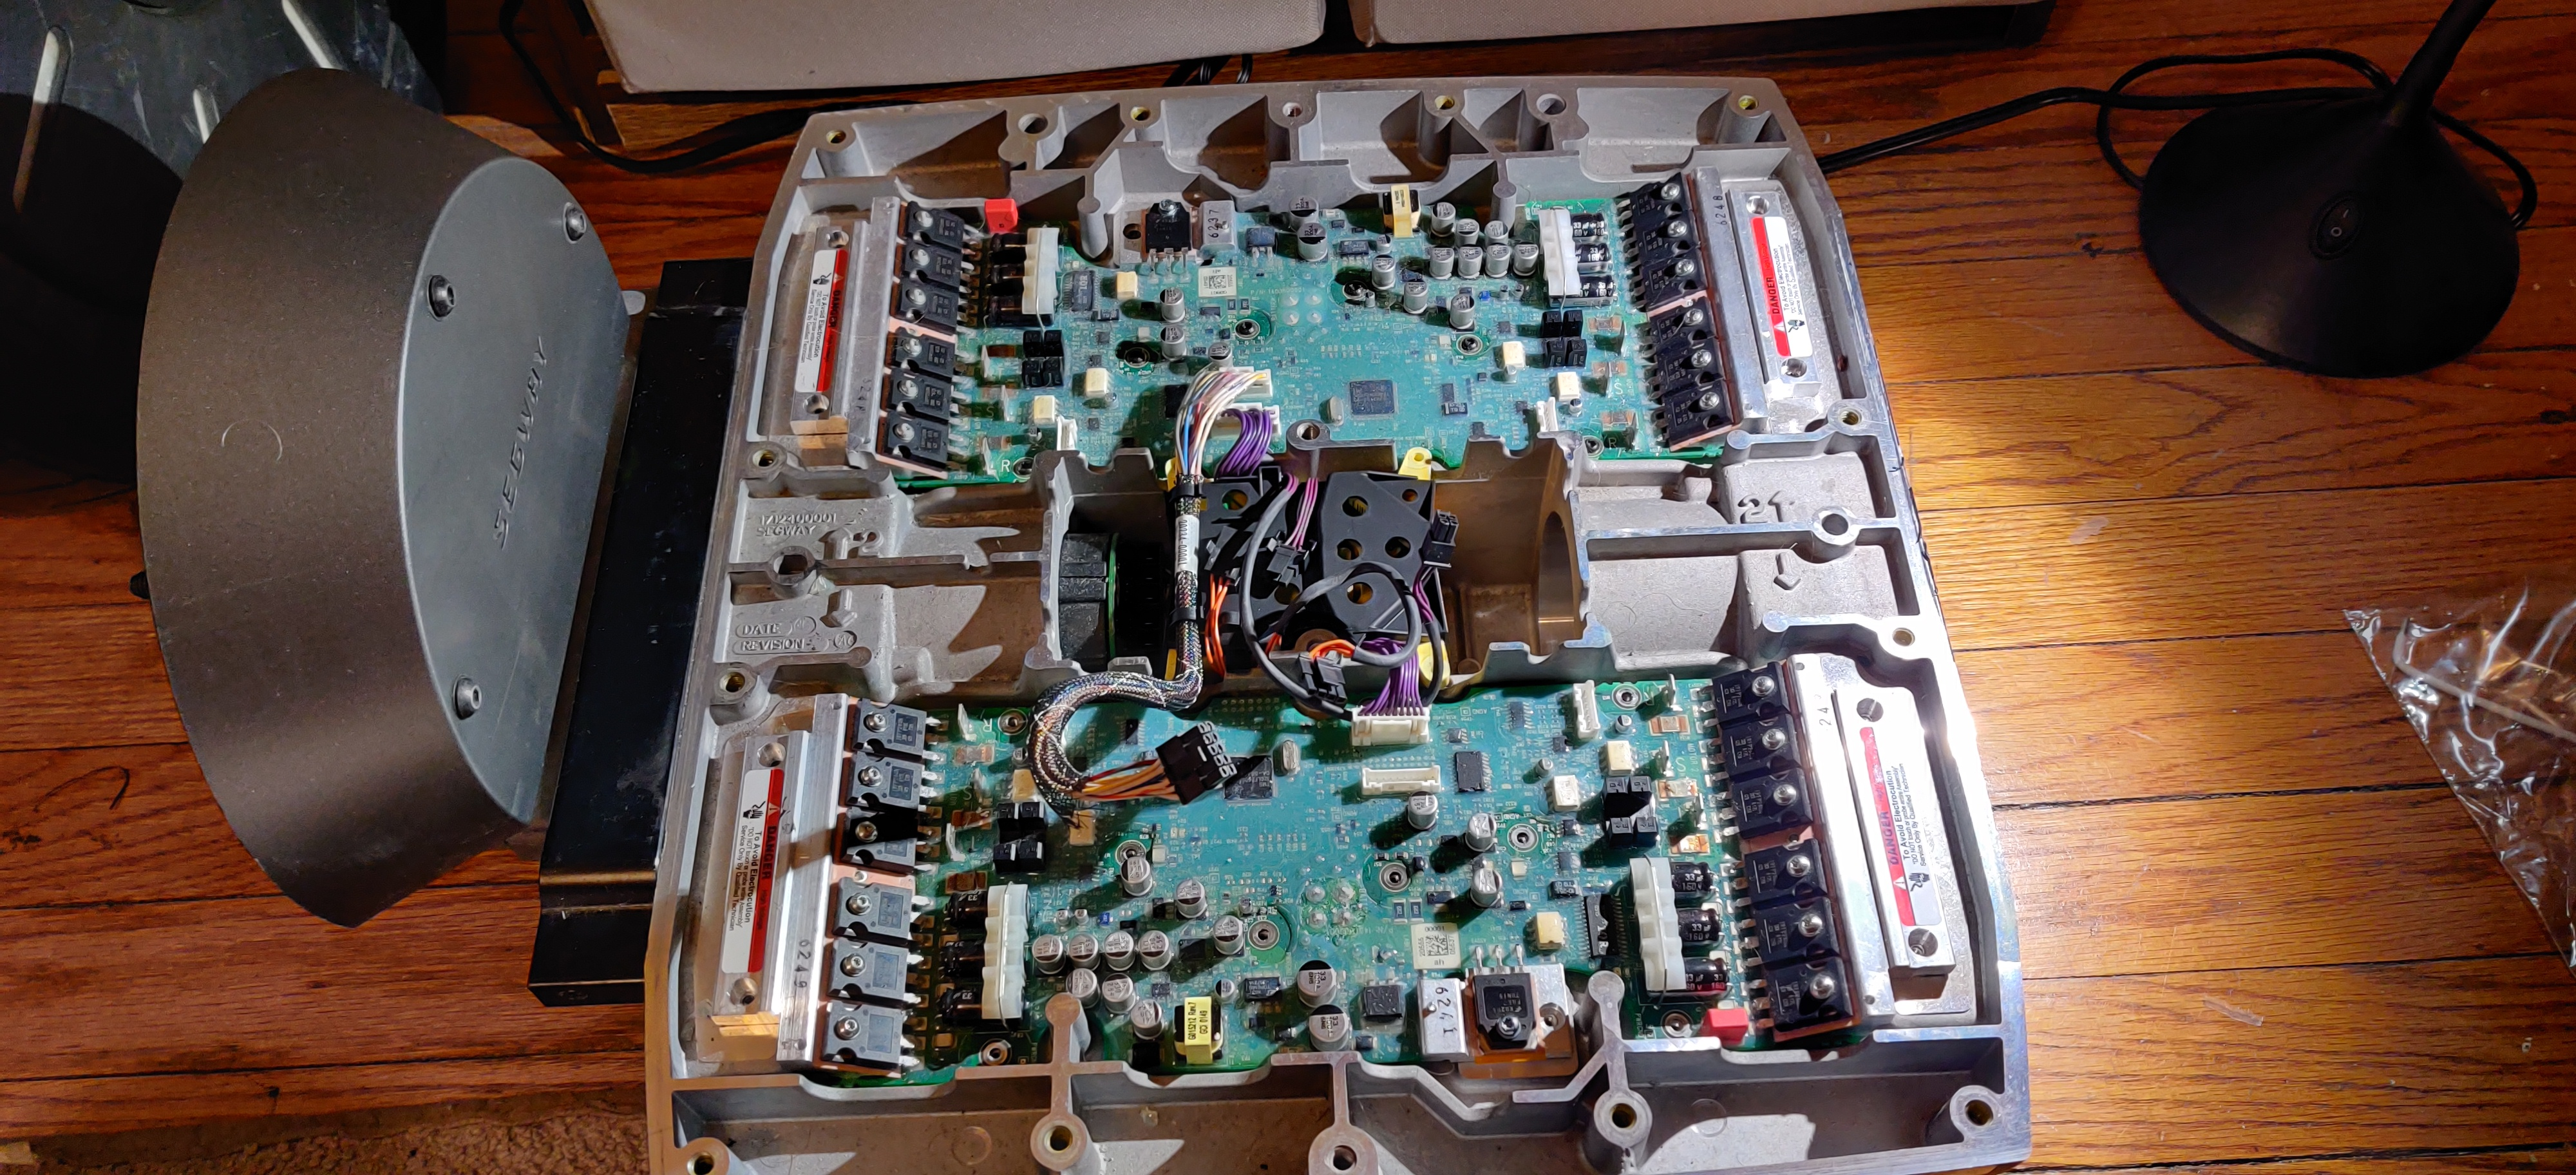
\includegraphics[]{segwayInternalsTop.jpg}
    \caption{caption}
    \label{fig:segwayInternalsTop.jpg}
\end{figure}

\begin{figure}
    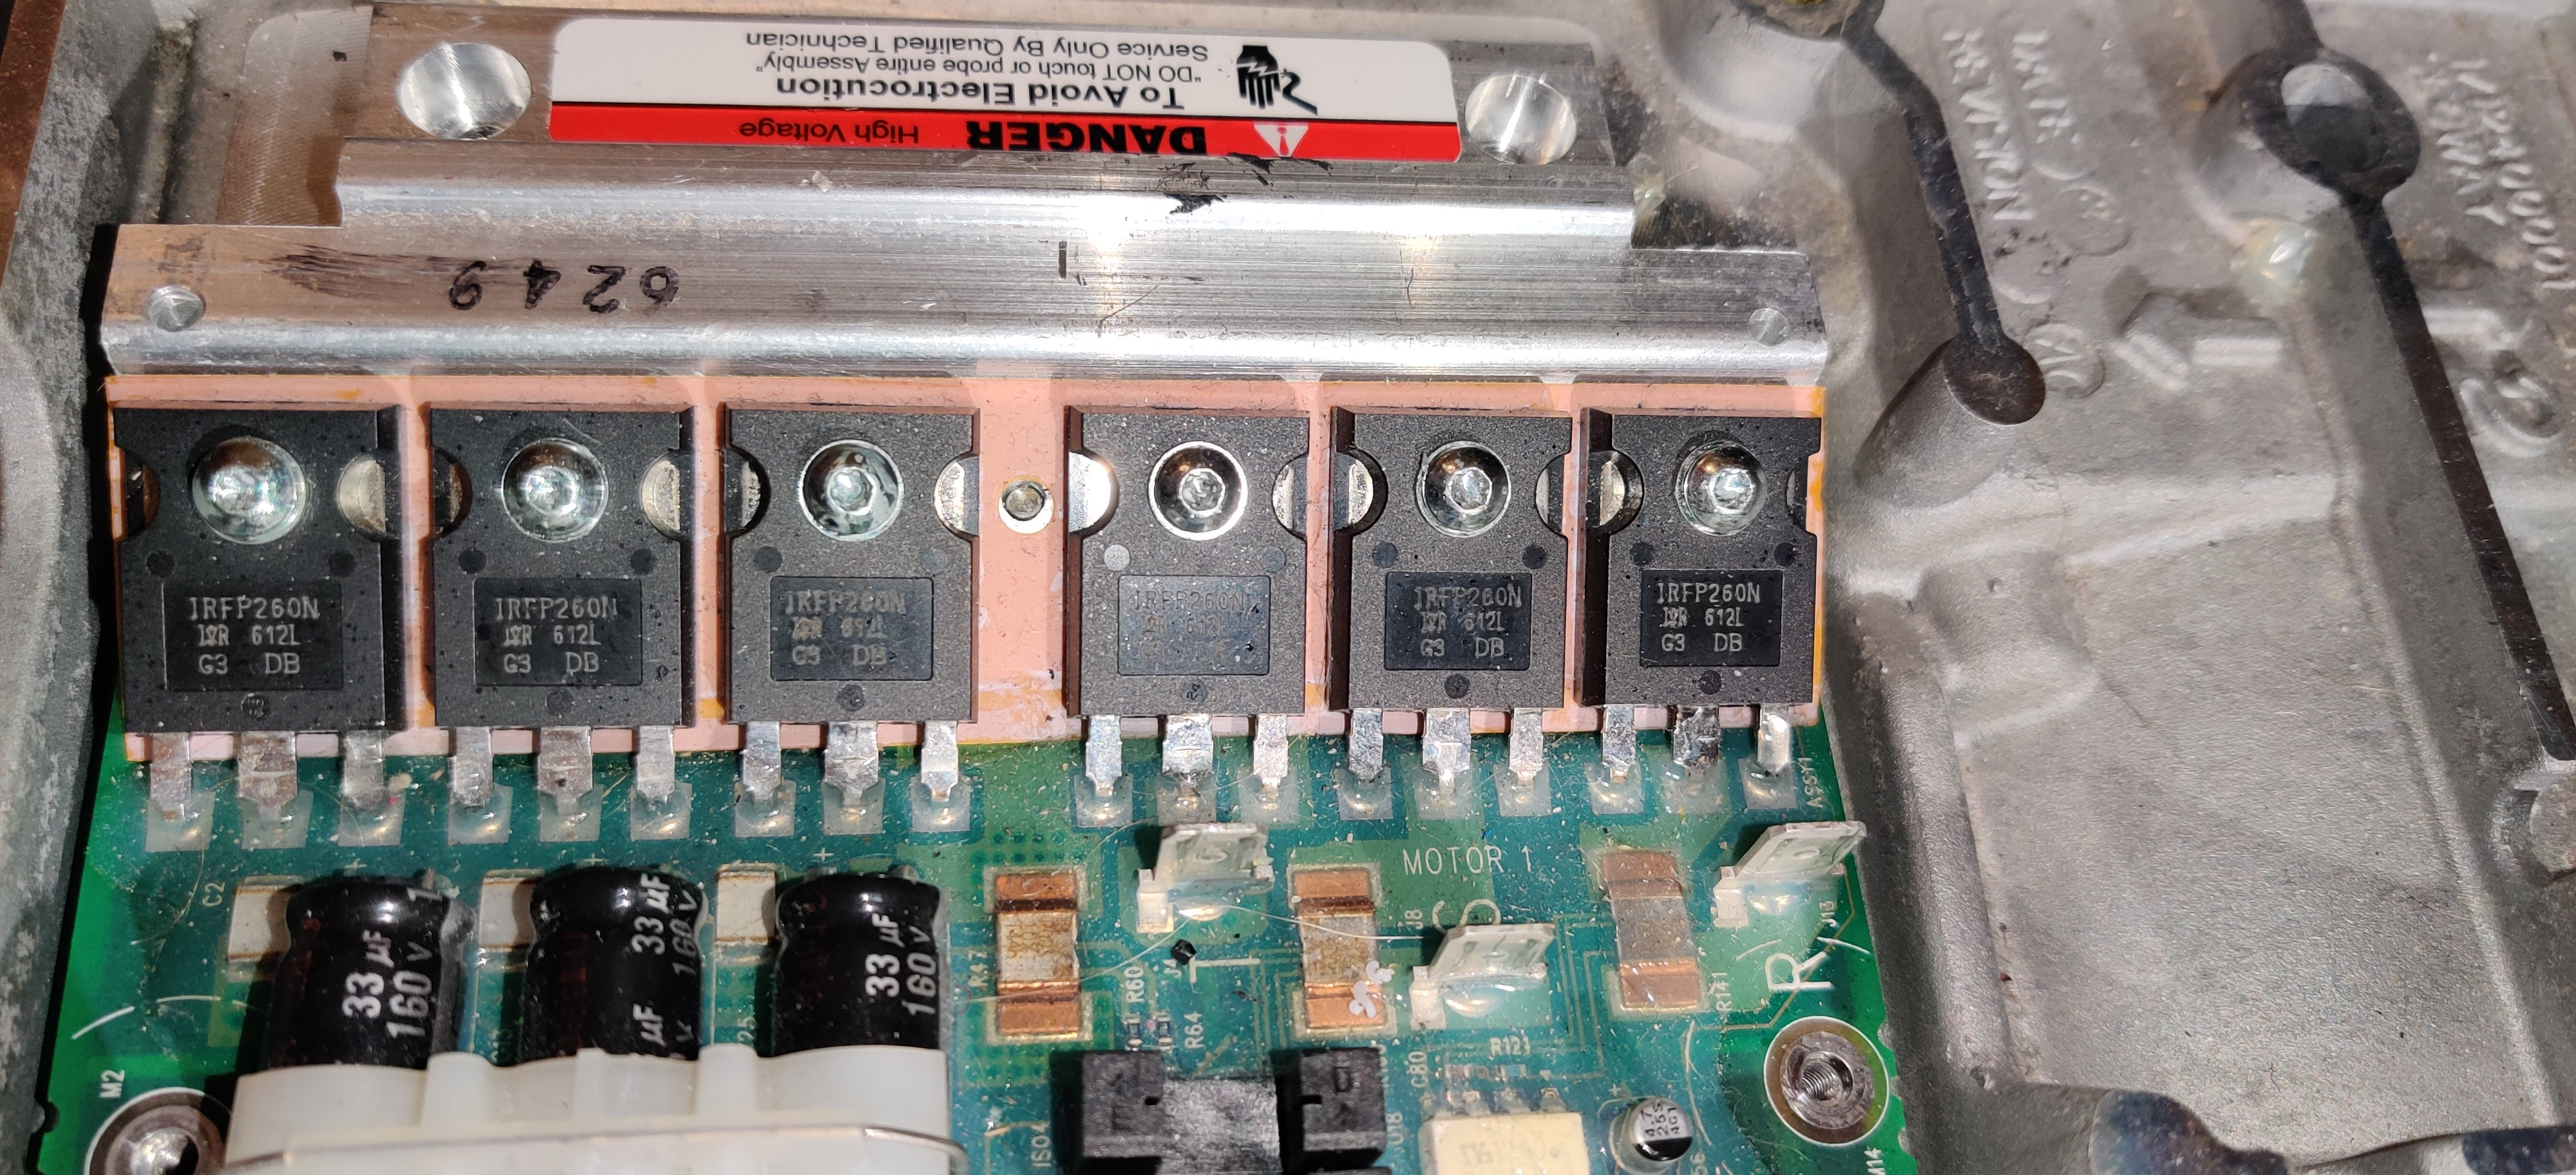
\includegraphics[]{segwayMotorDrivers.jpg}
    \caption{caption}
    \label{fig:segwayMotorDrivers.jpg}
\end{figure}

\begin{figure}
    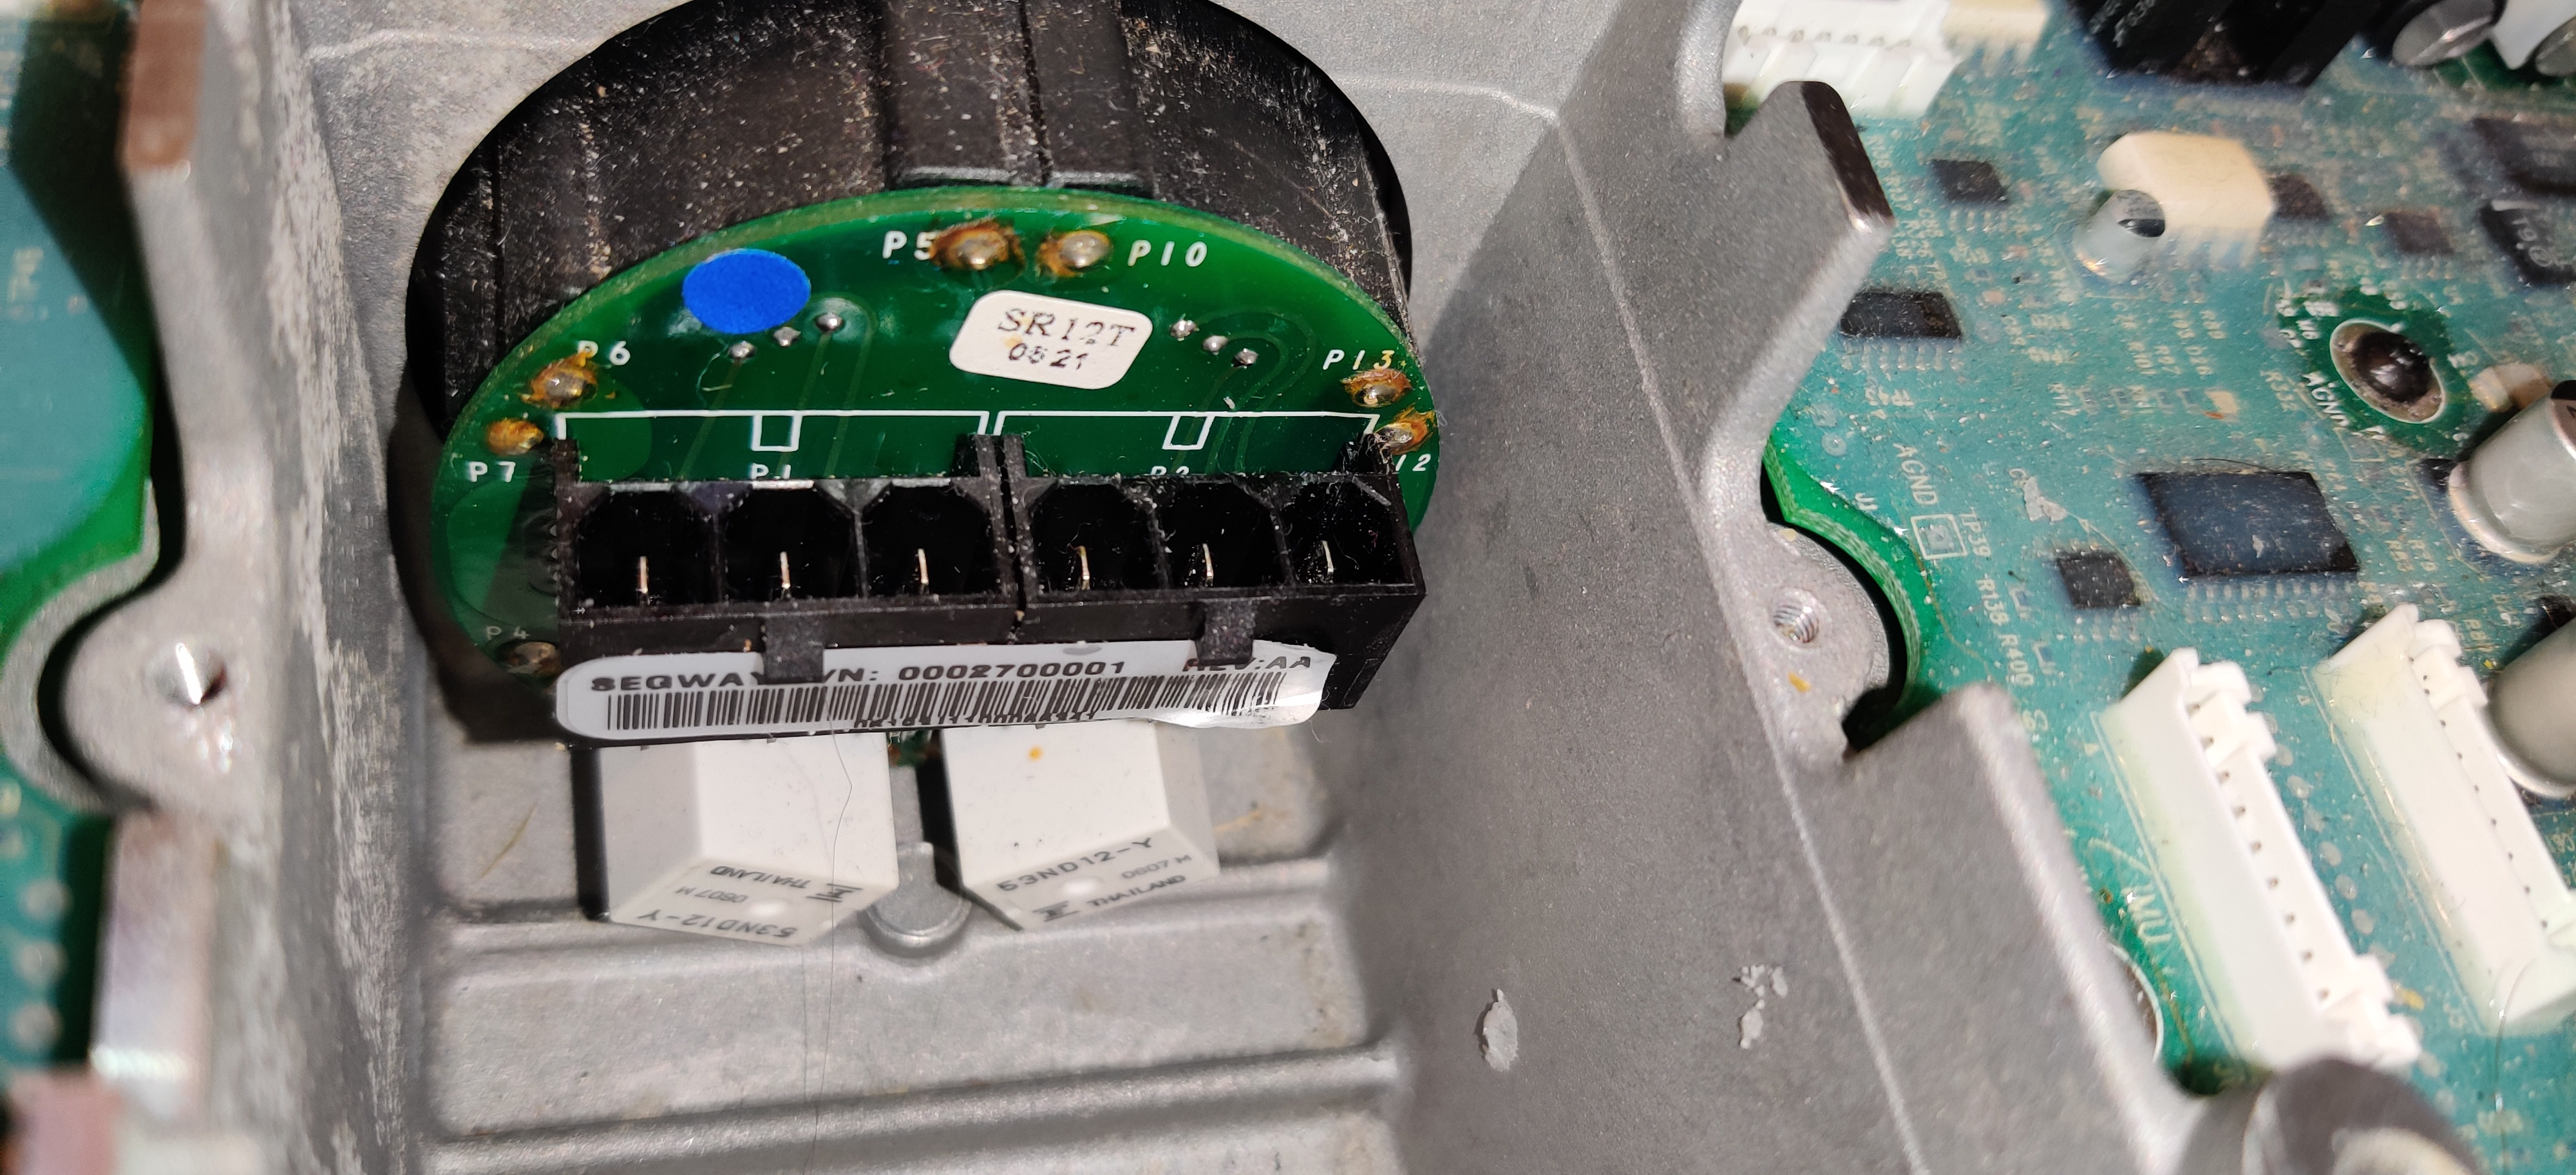
\includegraphics[]{segwayMotorInternal.jpg}
    \caption{caption}
    \label{fig:segwayMotorInternal.jpg}
\end{figure}

\begin{figure}
    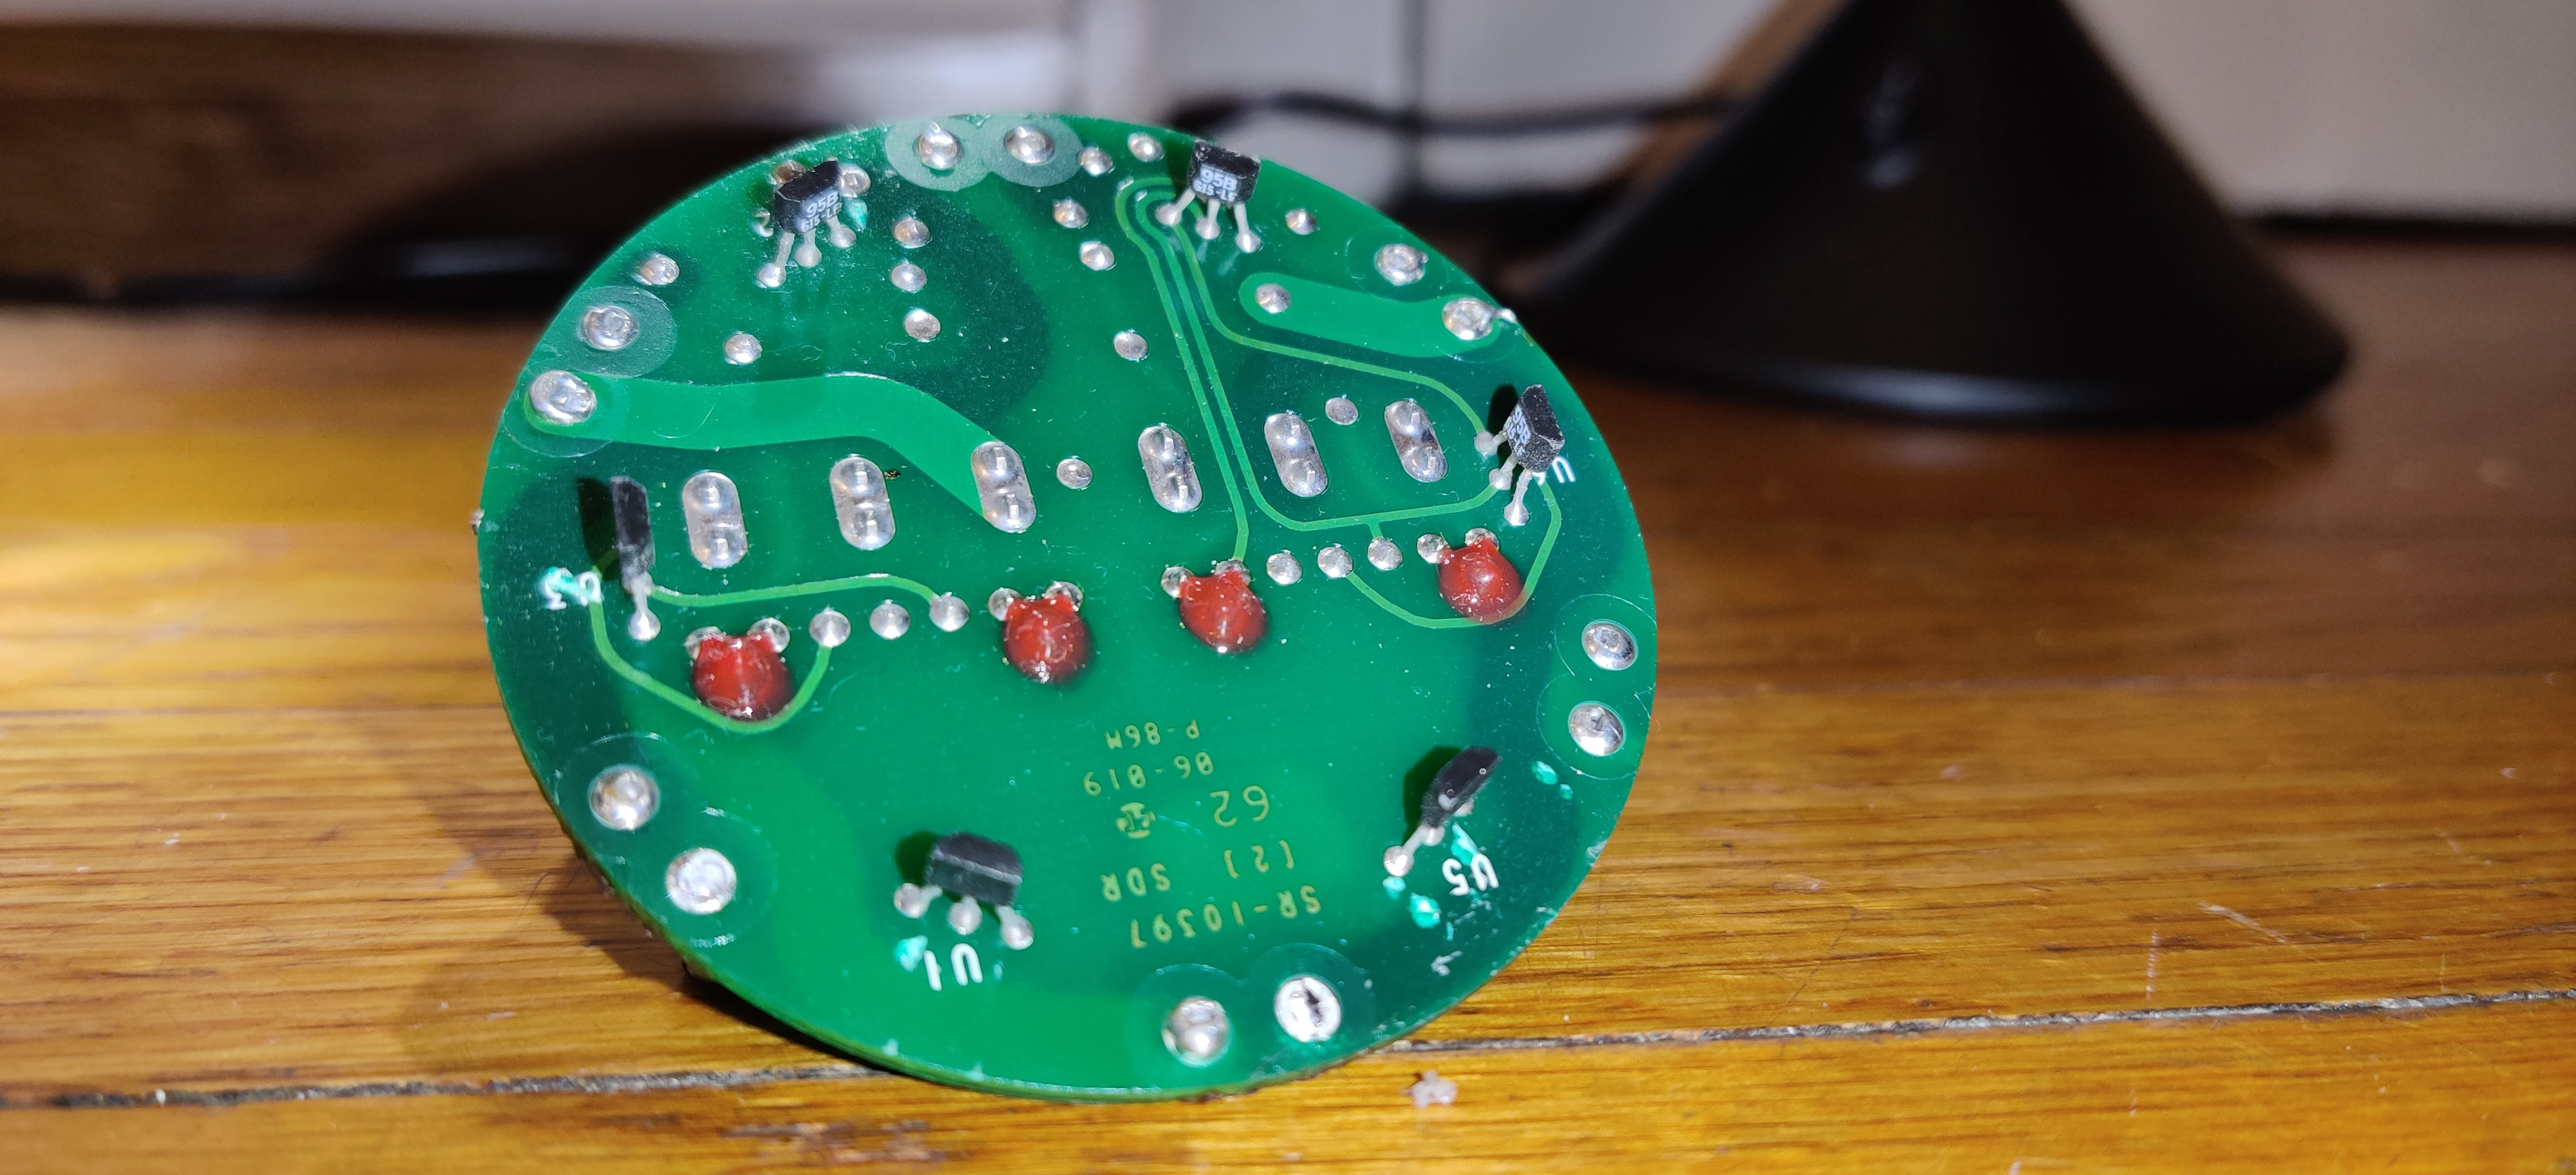
\includegraphics[]{segwayMotorPCBRear.jpg}
    \caption{caption}
    \label{fig:segwayMotorPCBRear.jpg}
\end{figure}

\begin{figure}
    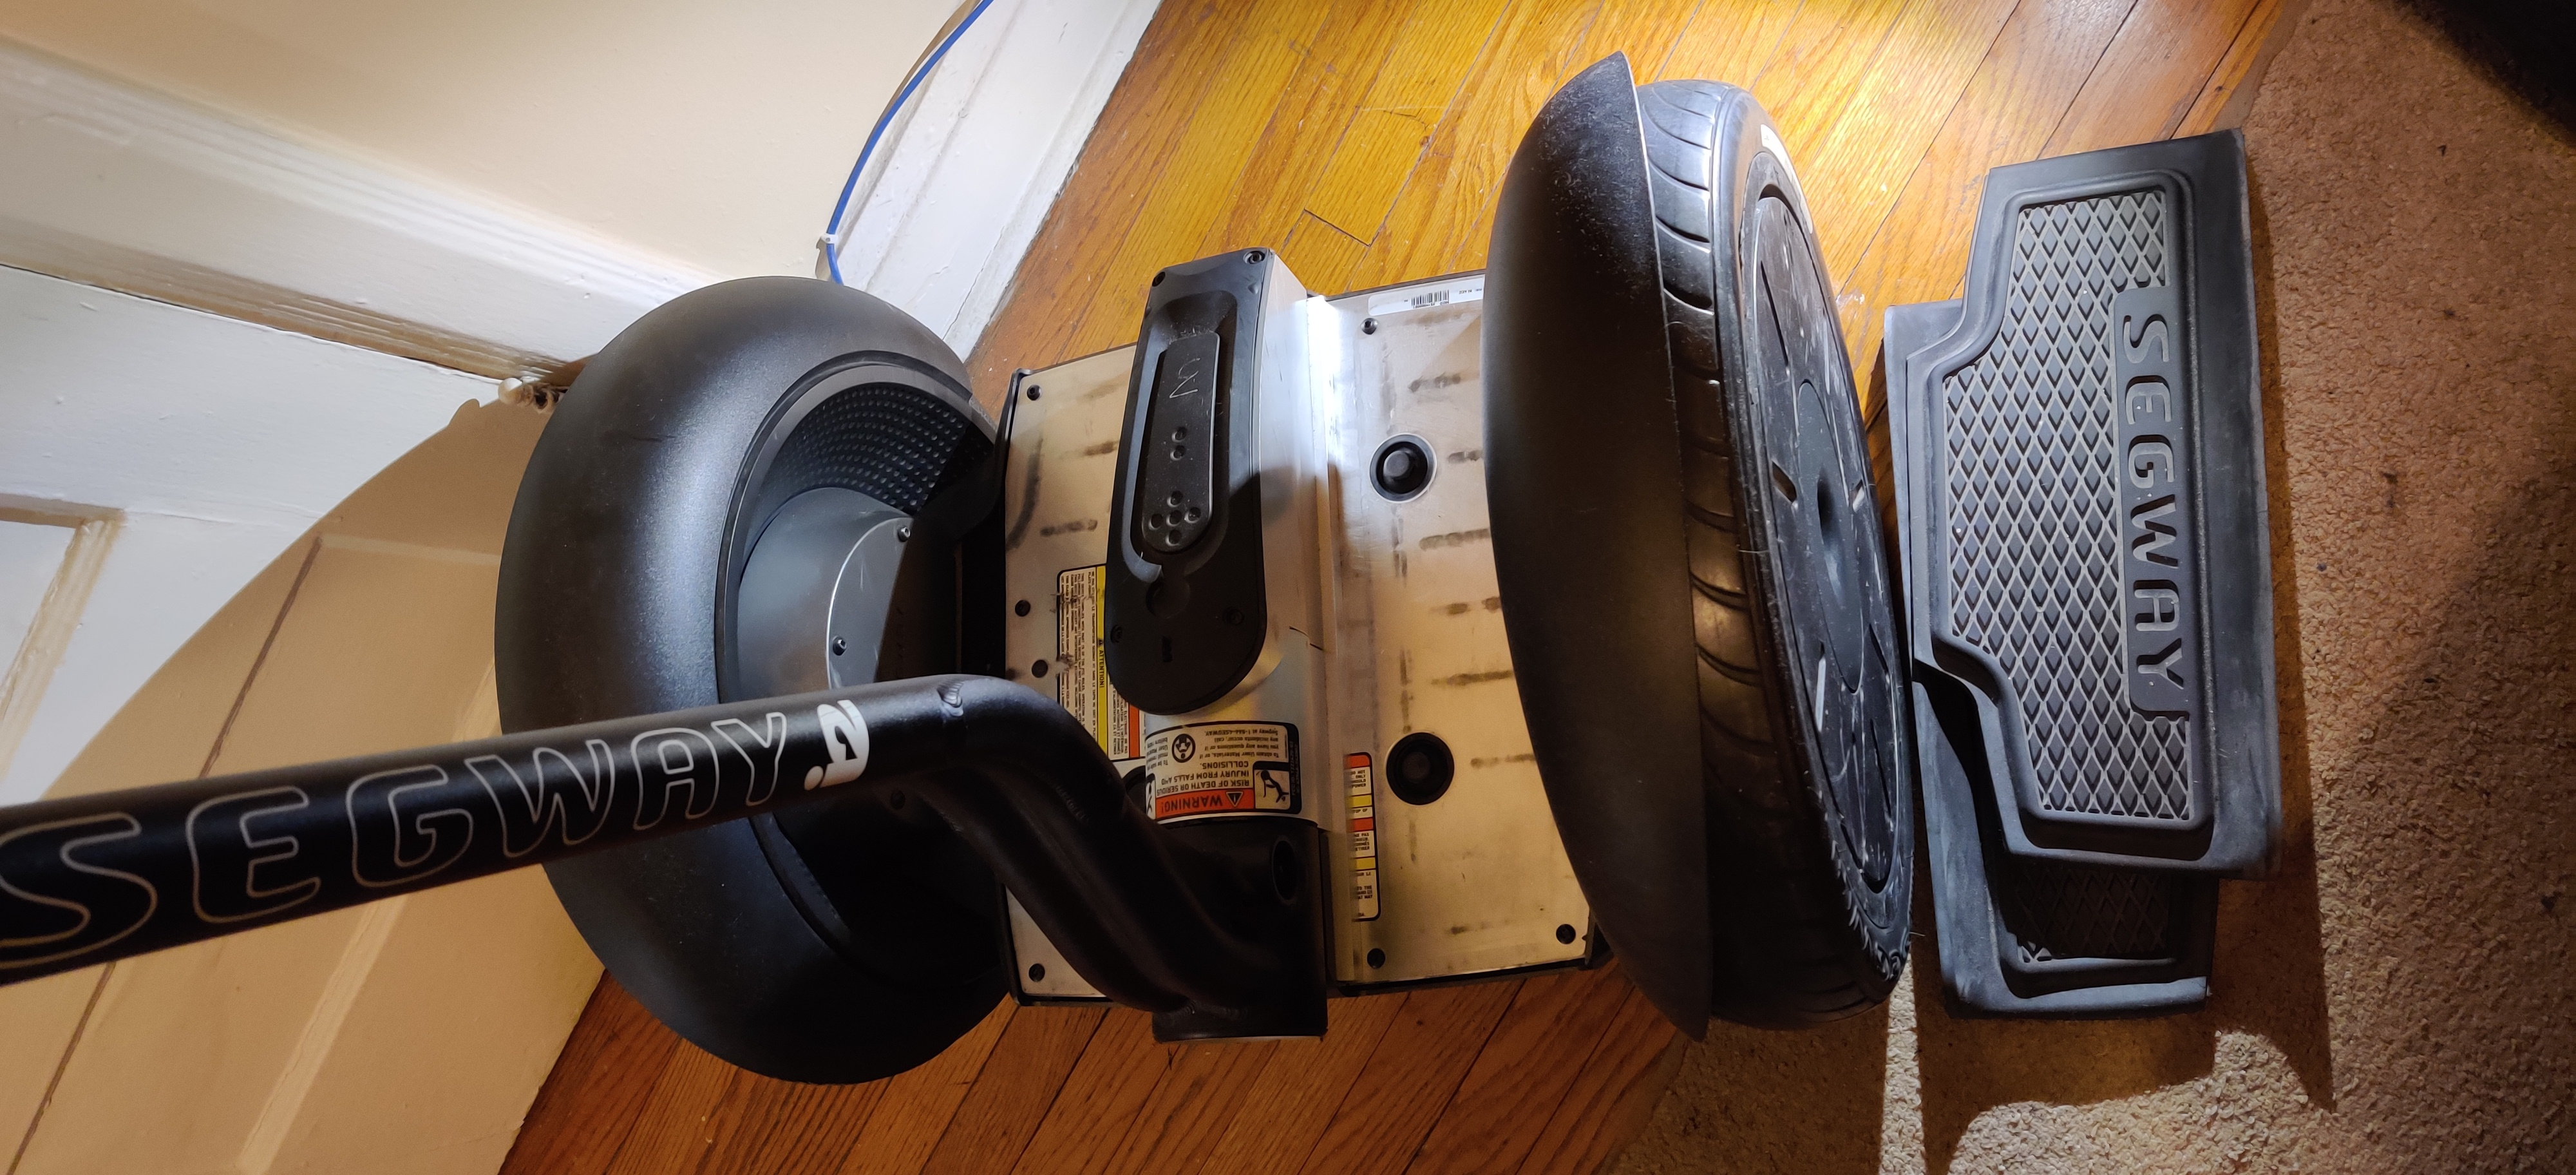
\includegraphics[]{segwayPadsRemoved.jpg}
    \caption{caption}
    \label{fig:segwayPadsRemoved.jpg}
\end{figure}

\begin{figure}
    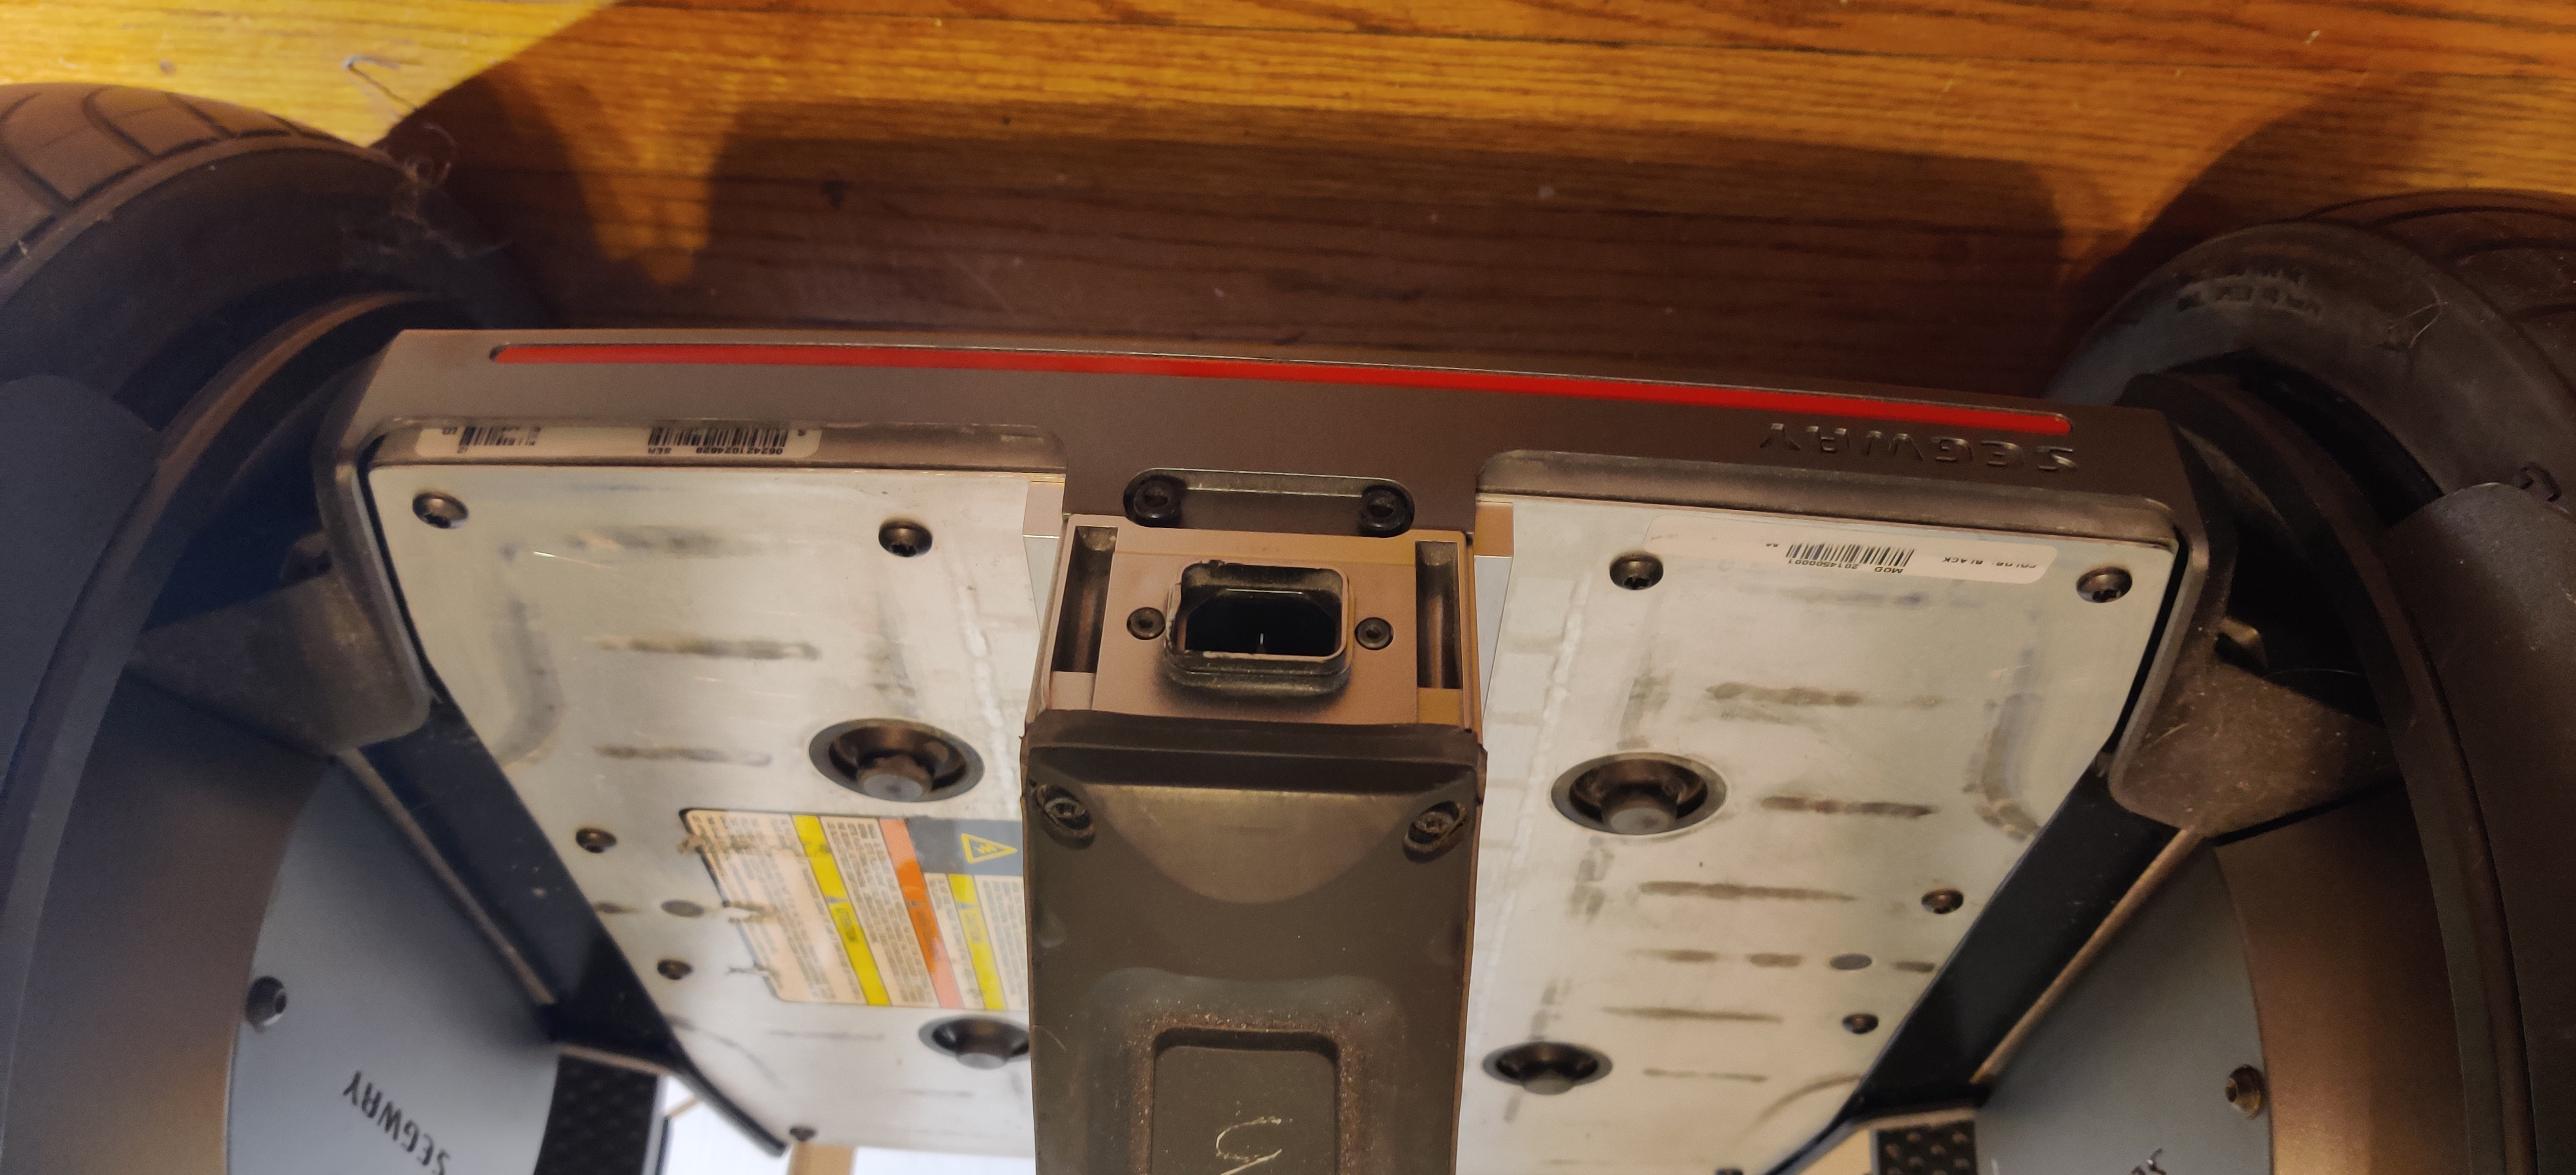
\includegraphics[]{segwayRear.jpg}
    \caption{caption}
    \label{fig:segwayRear.jpg}
\end{figure}

\begin{figure}
    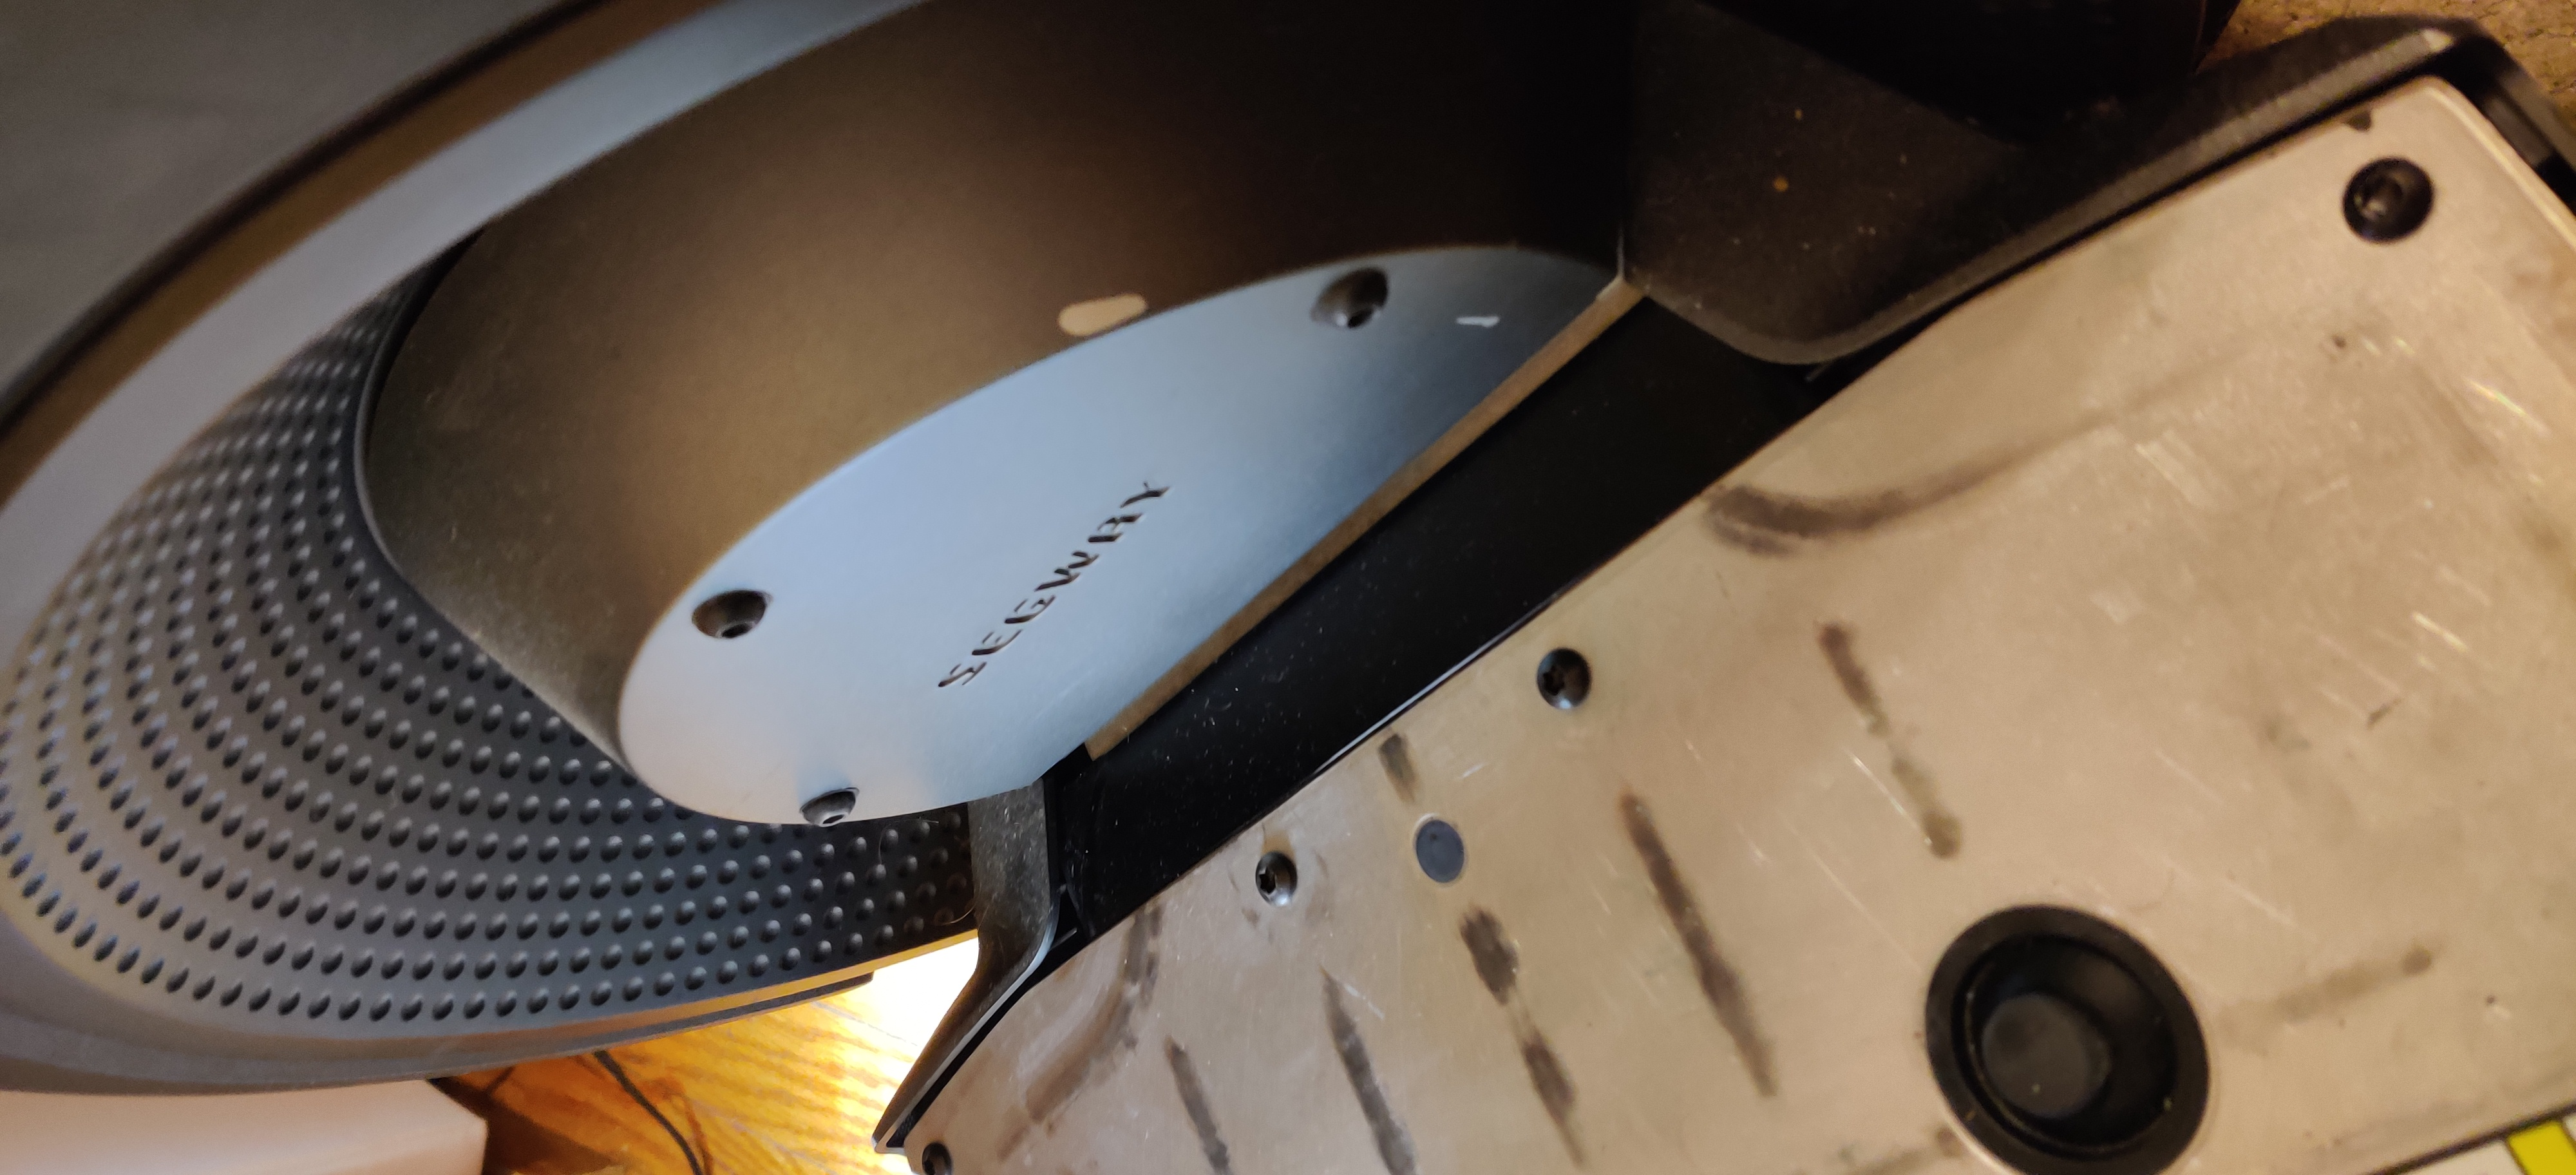
\includegraphics[]{segwayWheelAttachment.jpg}
    \caption{caption}
    \label{fig:segwayWheelAttachment.jpg}
\end{figure}

\begin{figure}
    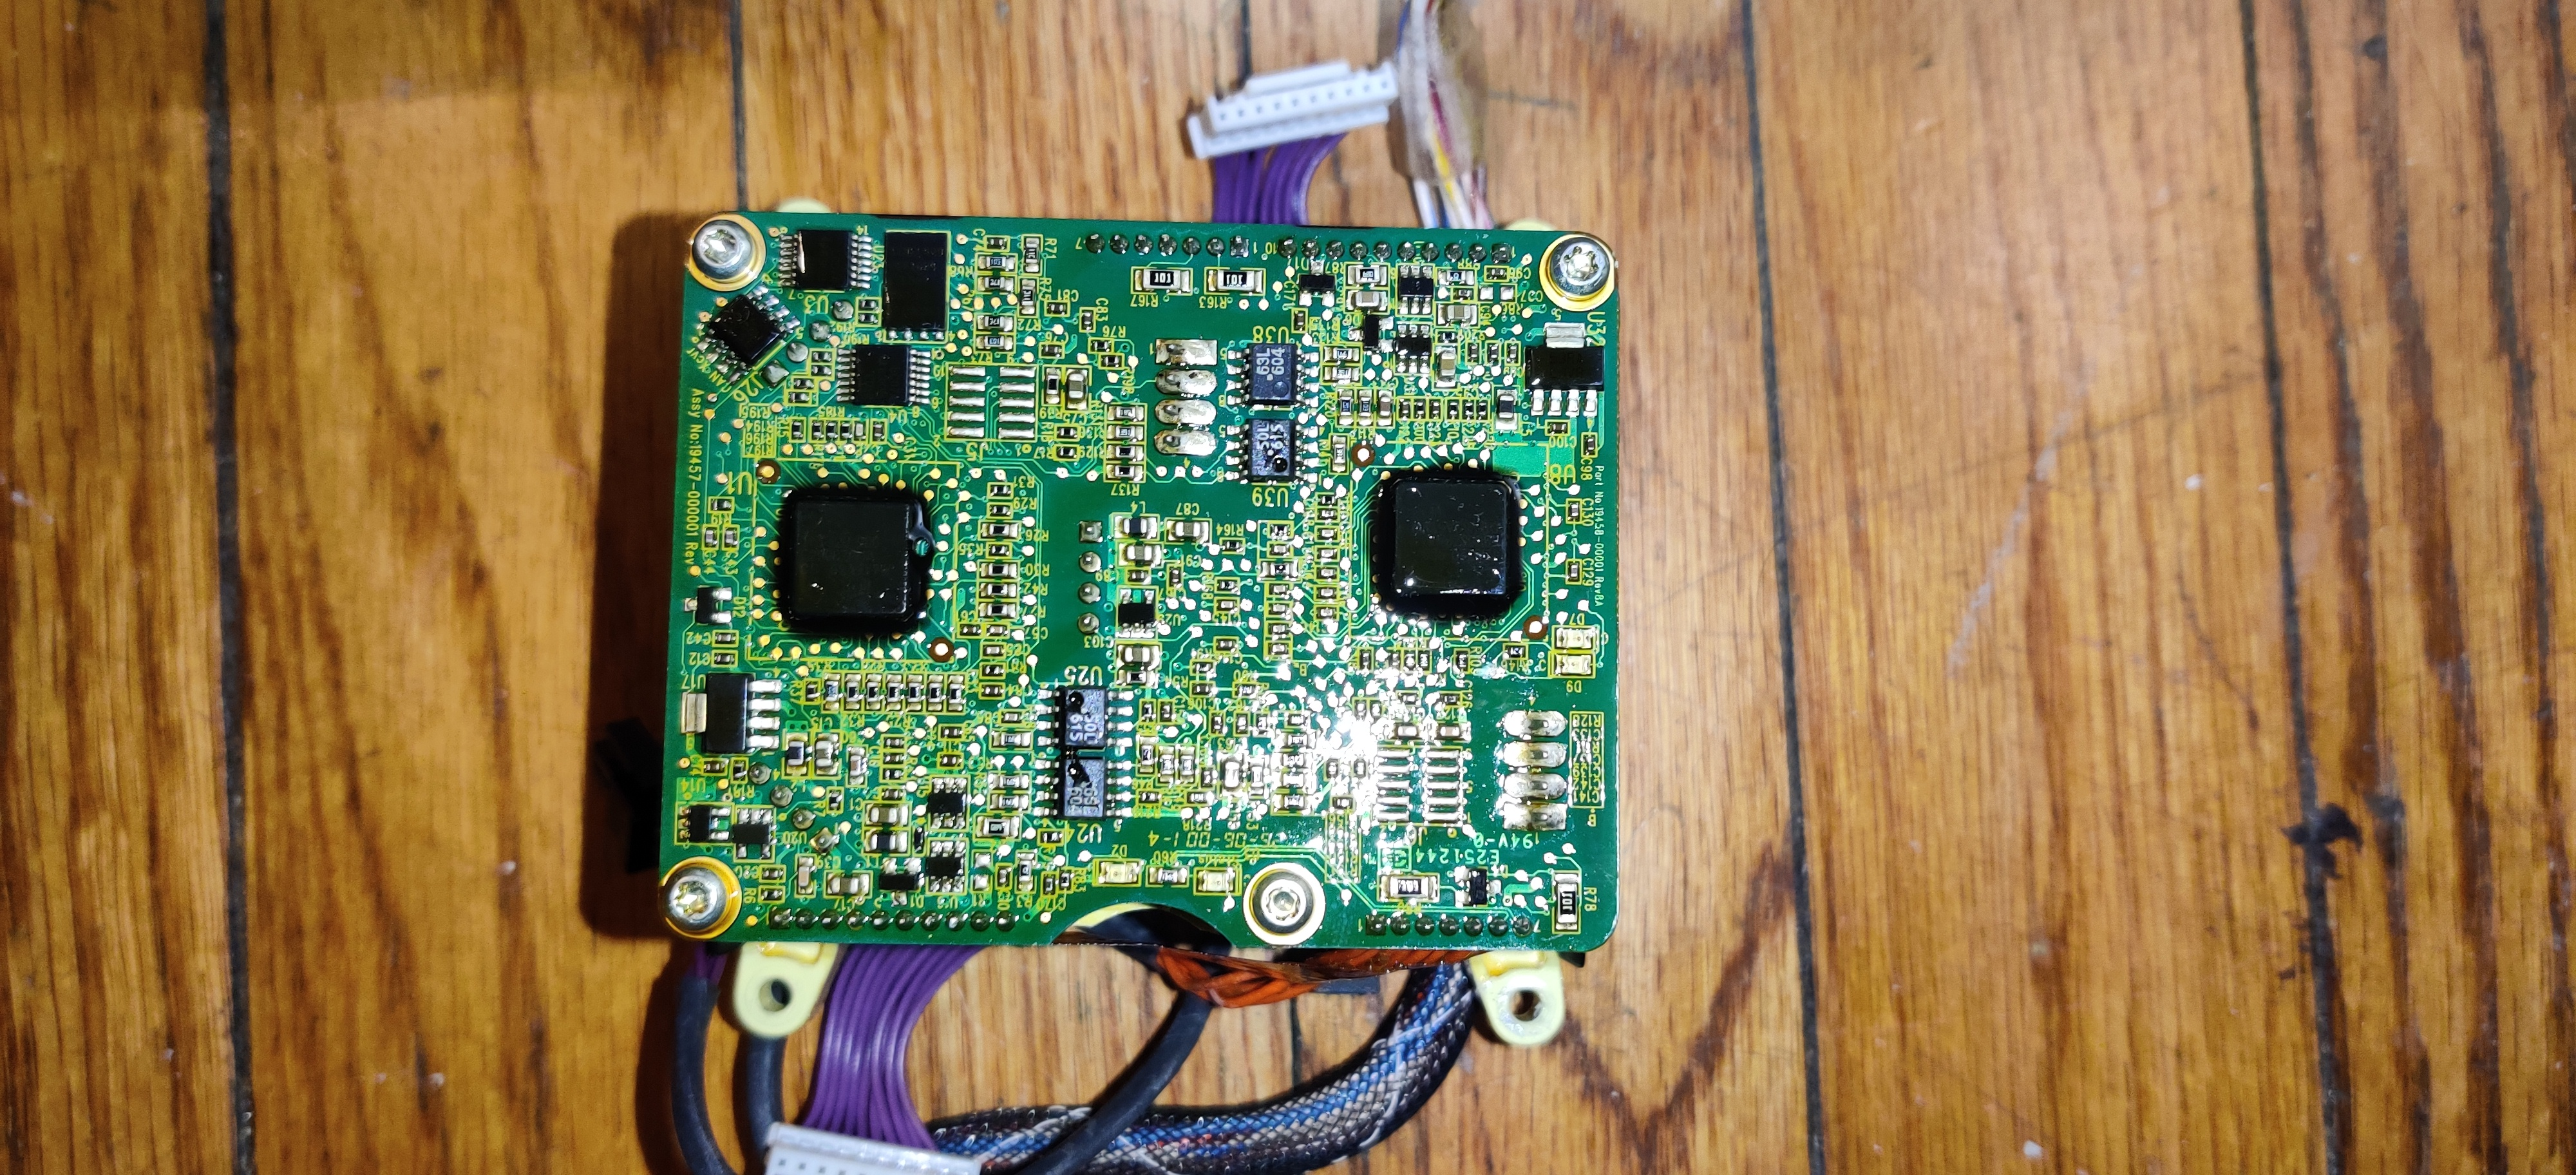
\includegraphics[]{segwayGyroCubeBottom.jpg}
    \caption{caption}
    \label{fig:segwayGyroCubeBottom.jpg}
\end{figure}

\begin{figure}
    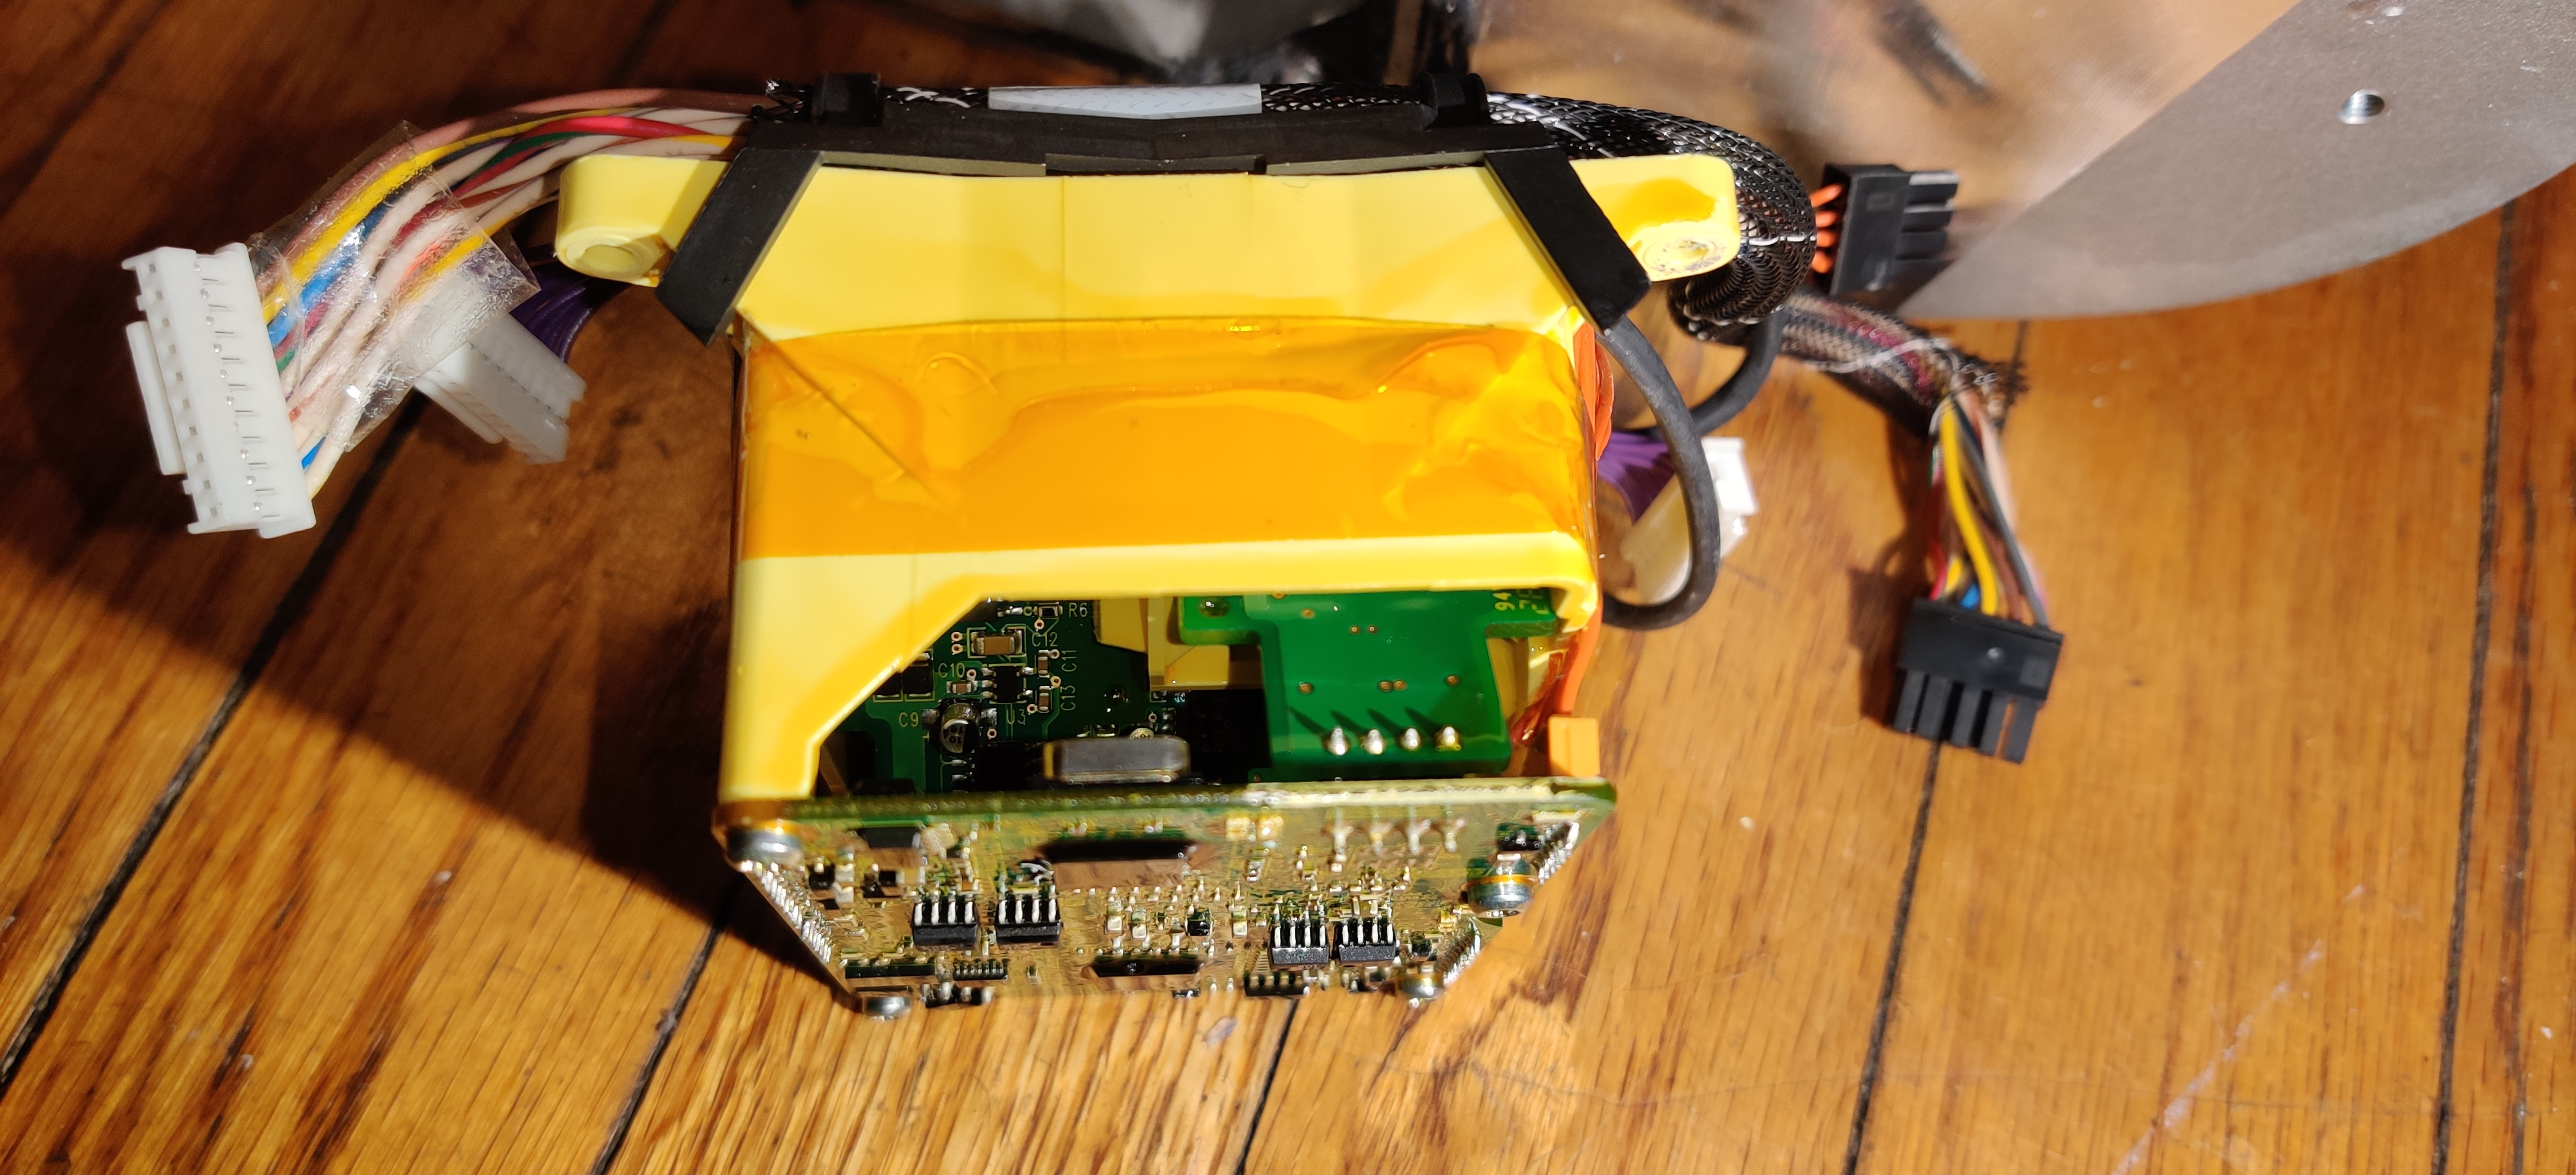
\includegraphics[]{segwayGyroCubeSide.jpg}
    \caption{caption}
    \label{fig:segwayGyroCubeSide.jpg}
\end{figure}

\begin{figure}
    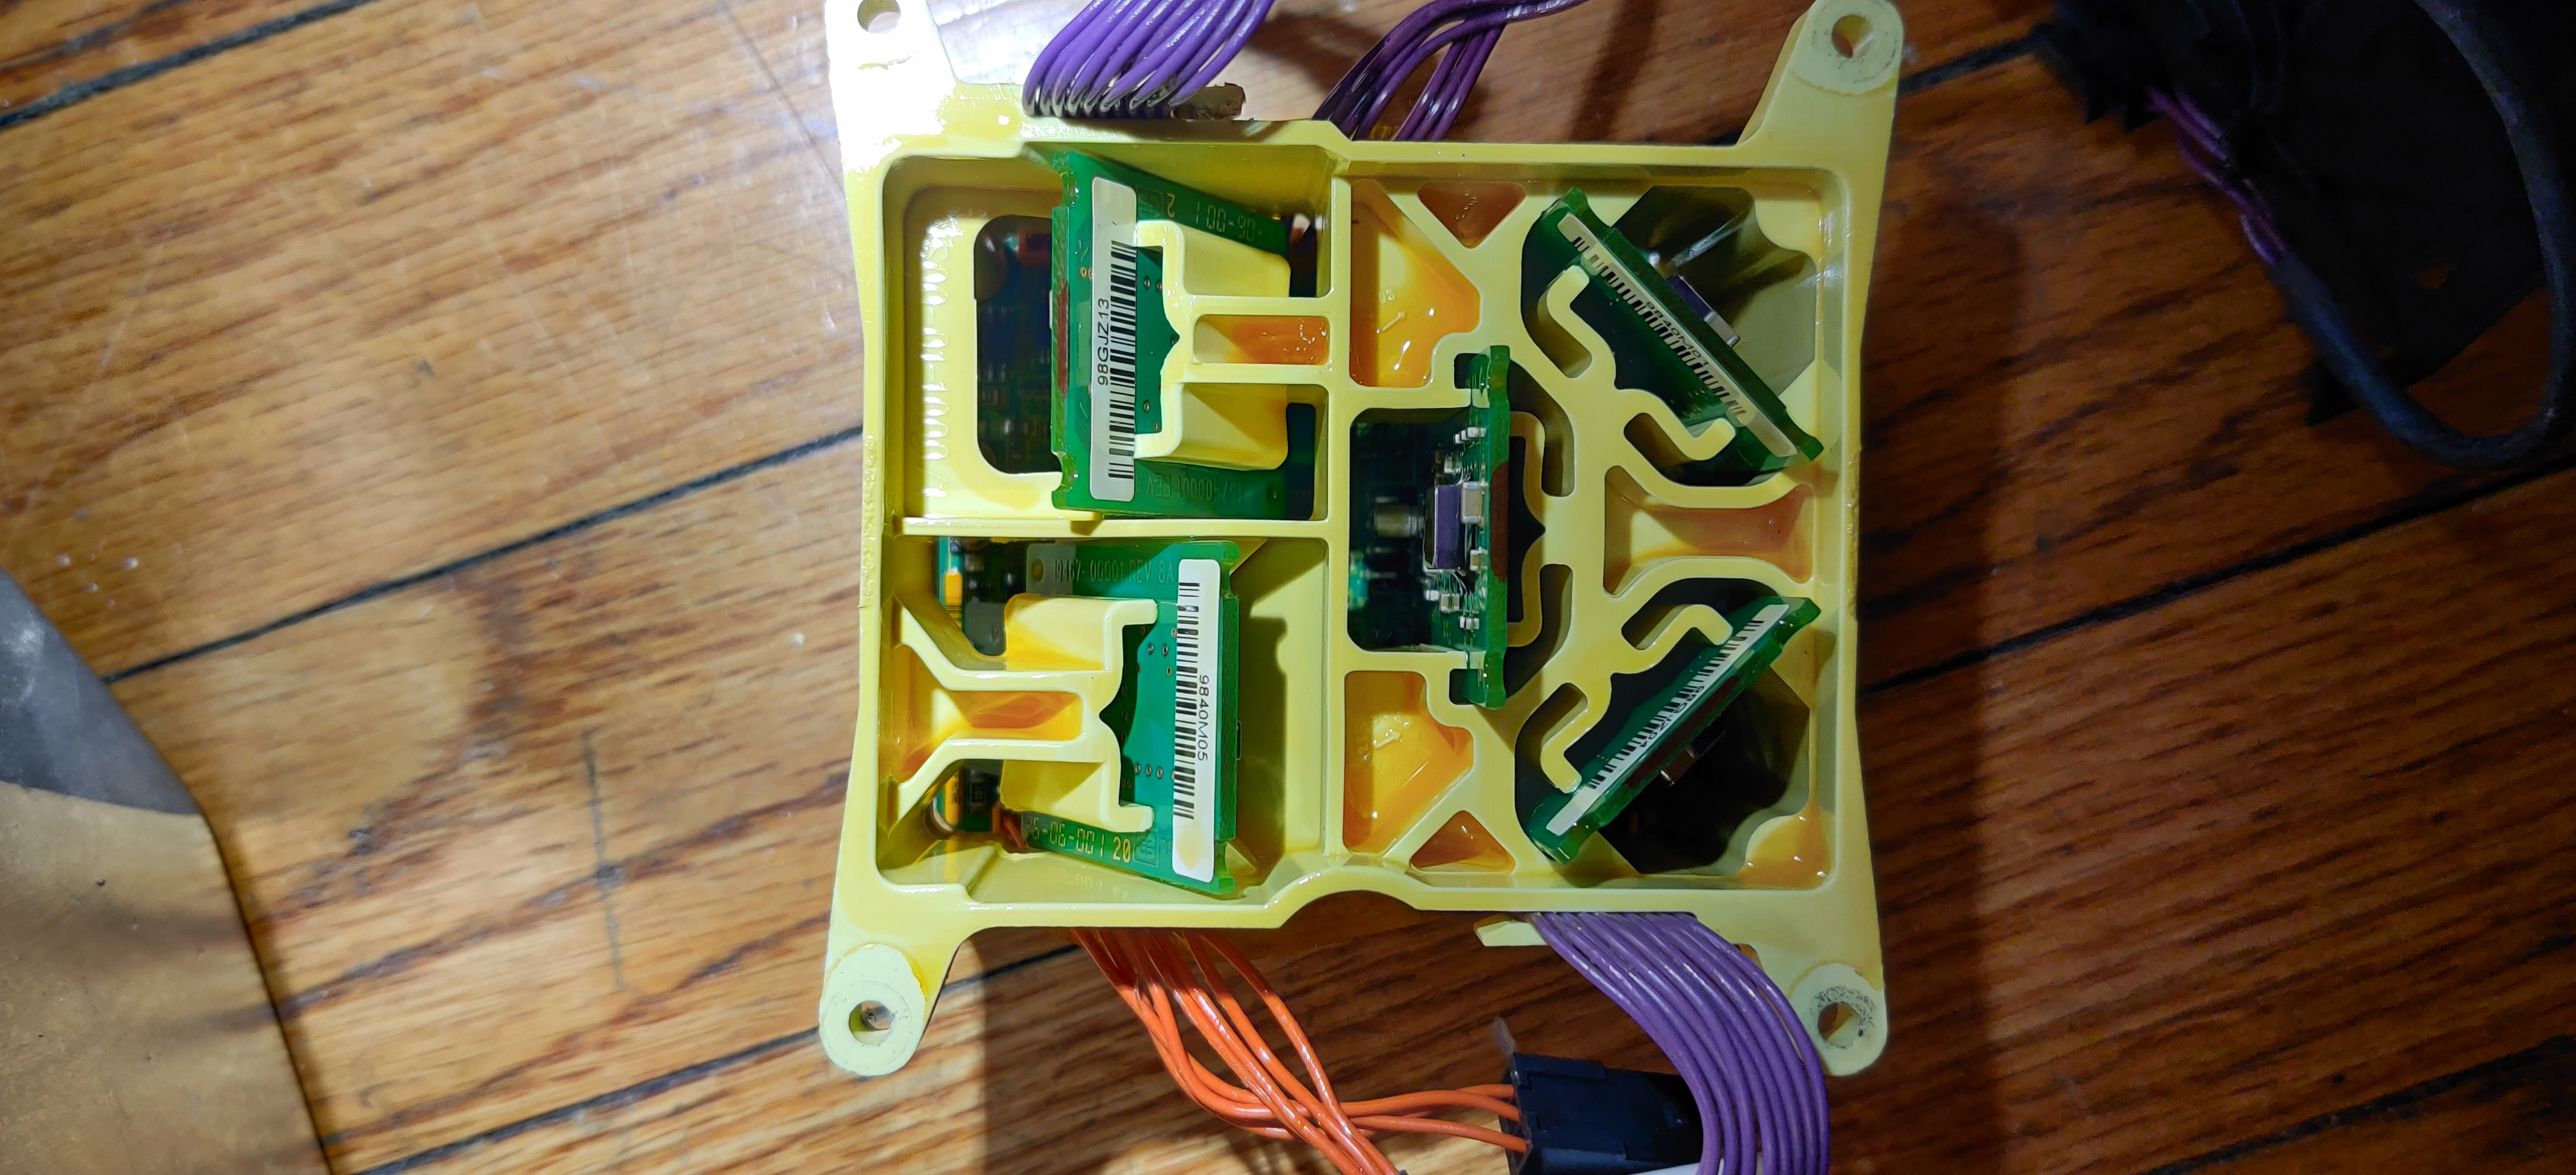
\includegraphics[]{segwayGyroCubeTop.jpg}
    \caption{caption}
    \label{fig:segwayGyroCubeTop.jpg}
\end{figure}

\end{document}